\documentclass[a4paper]{article}

% Set for specific document
\def\DOCTITLE{
  The Application of Robust Analysis Methods on Sparse Data for Mass-Resolved
  Neutron Spectroscopy}
\def\DOCAUTHOR{Daniel Nixon (120263697)}
\def\DOCDATE{\today}

% Set document attributes
\title{\DOCTITLE}
\author{\DOCAUTHOR}
\date{\DOCDATE}

\usepackage{fullpage}
\usepackage{scrextend}
\usepackage{titlesec}
\usepackage{fancyhdr}
\usepackage{hyperref}
\usepackage[style=numeric-comp,natbib=true]{biblatex}
\usepackage[nonumberlist,nopostdot]{glossaries}
\usepackage{glossary-mcols}
\usepackage[section]{placeins}
\usepackage{subcaption}
\usepackage{minted}
\usepackage{enumitem}
\usepackage[toc,page]{appendix}
\usepackage{booktabs}

% Handle graphics correctly
\ifx\pdftexversion\undefined
\usepackage[dvips]{graphicx}
\else
\usepackage[pdftex]{graphicx}
\DeclareGraphicsRule{*}{mps}{*}{}
\fi
\usepackage{rotating}

\addbibresource{DanNixon_Dissertation.bib}

% Deeply nested lists
\setlistdepth{9}
\setlist[itemize,1]{label=$\bullet$}
\setlist[itemize,2]{label=$\bullet$}
\setlist[itemize,3]{label=$\bullet$}
\setlist[itemize,4]{label=$\bullet$}
\setlist[itemize,5]{label=$\bullet$}
\setlist[itemize,6]{label=$\bullet$}
\setlist[itemize,7]{label=$\bullet$}
\setlist[itemize,8]{label=$\bullet$}
\setlist[itemize,9]{label=$\bullet$}
\renewlist{itemize}{itemize}{9}

% Setup headers and footers
\pagestyle{fancy}
\lhead{}
\chead{}
\rhead{\DOCDATE}
\rfoot{\thepage}
\cfoot{}
\lfoot{\DOCAUTHOR}

% Set header and footer sizes
\renewcommand{\headrulewidth}{0.1pt}
\renewcommand{\footrulewidth}{0.1pt}
\setlength{\headheight}{12pt}
\setlength{\headsep}{12pt}

% New page for each section
\newcommand{\sectionbreak}{\clearpage}

\newcommand{\chem}[1]{$\mathrm{#1}$}

% Glossary
\setglossarystyle{altlist}
\makeglossaries

\newacronym{MANTID}{MANTID}
  {Manipulation and Analysis Toolkit for Instrument Data}
\newacronym{RAL}{RAL}
  {Rutherford Appleton Laboratory}
\newacronym{IA}{IA}
  {Impulse Approximation}
\newacronym{YAP}{YAP}
  {Yttrium Aluminium Perovskite}
\newacronym{NCS}{NCS}
  {Neutron Compton scattering}
\newacronym{FSE}{FSE}
  {Final State Effects}
\newacronym{FWHM}{FWHM}
  {Full Width Half Maxima}
\newacronym{HWHM}{HWHM}
  {Half Width Half Maxima}
\newacronym{FABADA}{FABADA}
  {Fitting Algorithm for Bayesian Analysis of DAta}

\begin{document}

\maketitle

\begin{abstract}
  VESUVIO is a one of a kind neutron spectrometer and diffractometer situated at
  the ISIS facility on the \gls*{RAL} site in Oxfordshire. Recent development to
  the physical instrument have seen orders of magnitude improvements in the
  quality of data produced by the instrument.

  This dissertation focuses on the analysis of data obtained from mass-resolved
  spectroscopic experiments, specifically extending the current analysis
  workflows to reduce the amount of human involvement required to analyse the
  data.

  This has been attempted through the use of the FABADA minimiser recently
  implemented within the Manipulation and Analysis Toolkit for Instrument Data
  (MANTID) framework to create a Bayesian model selection algorithm based on a
  selection of models created through inspection of mass peaks present in an
  experimental spectrum.
\end{abstract}

\newpage

\renewcommand{\abstractname}{Declaration}
\begin{abstract}
  I declare that this dissertation represents my own work except where otherwise
  stated.
\end{abstract}

\renewcommand{\abstractname}{Acknowledgements}
\begin{abstract}
  I would like to thank my supervisor Dr. Paolo Zuliani for his guidance
  throughout the project as well as Dr. Matthew Krzystyniak for his valuable
  scientific input.
\end{abstract}

\tableofcontents

\section{Introduction}
\label{sec:introduction}

The subject of this dissertation is centred around the analysis of experimental
neutron scattering data produced by the VESUVIO instrument (see
\ref{sec:the_vesuvio_instrument}).

The work undertaken is part of an initiative to improve the data reduction and
analysis workflows for this unique instrument, which for the majority of the
life of the instrument have existed as a collection of proprietary FORTRAN
routines, only recently being ported into the widely used \gls*{MANTID} data
analysis tooklit.

Parts of this work follow on from work that I undertook during my placement year
at the ISIS facility in Oxfordshire which are described in detail in
\cite{Nixon2015}.

Recent improvements made to the VESUVIO instrument have allowed the duration of
a single run to be significantly reduced, as such the volume of data produced
by the instrument per operational cycle of the ISIS facility is growing.

This increased volume of data therefore increased the time taken to process the
data as each experiment will require a new driver script to be created for the
specific sample, which may then require testing several times in order to tune
parameters, such as the intensity constraints, to obtain the best fit of the
defined model to the experimental spectrum.

An ideal solution would be that which allows the analysis jobs to be
automatically executed as the data is produced by the instrument, taking into
account that a single experiment may involve multiple runs (data files) for
example in the case where an experiment is performed over a range of sample
temperatures.

This is a solution used by several other instruments at the ISIS facility using
the recently released auto-reduction service, however currently this is not a
feasible option for VESUVIO due to; the reliance on the scientist to define the
fitting model, the need to verify the model and parameters and the computational
cost of running the current analysis.

This project will aim to address only the first point; the need to manually
define the fitting model. This ill be done through the use of Bayesian model
selection in which the most appropriate fitting model is selected based on the
probability of its hypothesis given the data.

As for the remaining two points; the computational cost can be addressed simply
through optimisation of the current workflow, for instance currently only one
thread is used to run the overall workflow (multiple threads are used during the
more expensive correction algorithms) however as described in section
\ref{sec:existing_data_analysis_workflow} the workflow operates by fitting each
spectrum in turn which is an obvious place to introduce multithreading due to
the isolation of data treatment per spectrum.

The need to manually verify the fitting model is a difficult requirement to
remove from any data analysis workflow, especially one in which the model is
derived through an automatic model selection scheme.

\subsection{Project Aim}
\label{sec:project_aim}

The aim of the project is to improve the existing data analysis workflow for the
VESUVIO instrument as implemented in the \gls*{MANTID} toolkit.

\subsection{Objectives}
\label{sec:objectives}

The objectives of the project can be summarised in two main areas:

\begin{itemize}
  \item
    Adding an additional fit function that allows fitting of the multivariate
    Gaussian Compton peak profile for anisotropic mass peaks, details of which
    are in section \ref{sec:multivariate_gaussian_fitting}

  \item
    Providing functionality to allow the peaks in a sample to automatically be
    assigned a mass, detailed in section \ref{sec:bayesian_analysis_routines}
\end{itemize}

\section{Background}
\label{sec:background}

This section describes the general background to the project. Information
specific to each feature implemented is provided in sections
\ref{sec:mvg_background} and \ref{sec:bayes_background} respectively.

\subsection{The VESUVIO instrument}
\label{sec:the_vesuvio_instrument}

VESUVIO is a one of a kind neutron spectrometer located in target station 1 of
the ISIS facility on the \gls*{RAL} site, Oxfordshire.

\begin{figure}[h!]
  \centering
  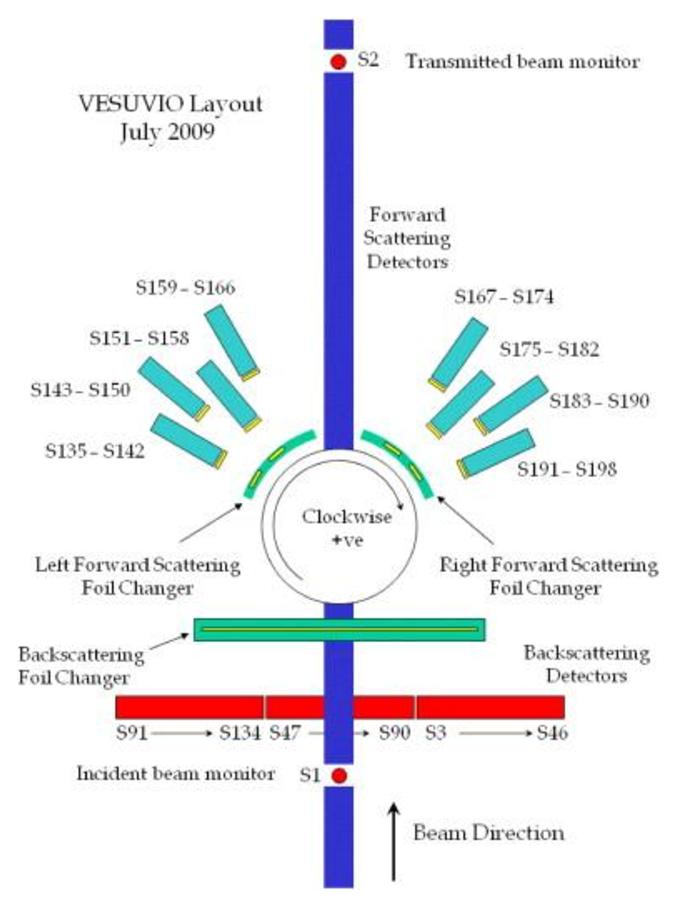
\includegraphics[width=0.5\textwidth]{graphics/evs_layout_july2009.eps}
  \caption{VESUVIO instrument layout \cite{Mayers2011}}
  \label{fig:vesuvio_layout}
\end{figure}
\FloatBarrier

The physical layout of the instrument is detailed by figure
\ref{fig:vesuvio_layout}.

The image shows the sample tank at the centre of the instrument through which
the beam is directed, two monitors are used to measure the beam intensity before
(S1) and after (S2) it has passed through the sample.

The forward scattering detectors are composed of eight banks of eight \gls*{YAP}
detectors which detect Gamma rays emitted by the gold foils directly in front of
the detectors when they absorb a neutron. Each bank is vertically arranged such
that there are four detectors on either side of the horizontal plane
\cite{Mayers2011}.

The backscattering detectors are in three banks of 44 $\mathrm(Li)^{6}$ doped
glass bead neutron detectors.

A measurement mode known as the foil cycling technique \cite{Schooneveld2006} is
employed on VESUVIO, whereby Gold foils are cycled in and out of the secondary
beam path between the sample and analyser/detector. This technique is
effectively a combination of the resonance detector and filter difference
measurement techniques which can also be configured on VESUVIO.

This technique is used to give improved resolution by narrowing the \gls*{FWHM}
of the energy transfer function. The final spectrum is given by subtracting the
foil in spectrum from the foil out spectrum.

VESUVIO operates using a technique known as \gls*{NCS} in which momentum
distributions are measured by means of inelastic neutron scattering. The
technique is similar to traditional Compton scattering in which the momentum of
electrons is measured by means of scattering high energy photons.

In principle VESUVIO operates as any other indirect inelastic neutron
spectrometer does in that neutrons are scattered by the sample then have their
momentum changed by an analyser bank (in the case of VESUVIO this is the gold
foils) and then hit a detector.

The initial stages of analysis are therefore identical to an indirect inelastic
spectrometer in that given the geometric and neutronic parameters of the
instrument the count rate at a given time can be calculated.

The count rate (measured by the detector) is given the standard expression
described by equation \ref{eq:countrate_tof} for an indirect geometry time of
flight spectrometer \cite{Windsor1986} for a system of $N$ identical atoms
scattering neurons into a detector at polar coordinates $d\Omega$ and $\theta$.

\begin{equation}
  \label{eq:countrate_tof_e0}
  E_{0}(E_{1}, t) =
    \frac{m}{2}
    \left(\frac{L_{0} v}{v_{1} t - L_{1}}\right)^{2}
\end{equation}

\begin{equation}
  \label{eq:countrate_tof}
  C(t) =
    2\left(\frac{2}{m}\right)^{\frac{1}{2}}
    \frac{E_{0}^{\frac{3}{2}}}{L_{0}}
    I(E_{0}) D(E_{R})
    N \frac{d^{2}\sigma}{d\Omega dE_{1}} d\Omega
\end{equation}

where; $m$ is the mass of a neutron, $E_{0}$ is the incident neutron energy,
$E_{1}$ is the final energy of scattered neutrons, $L_{0}$ is the length of the
incident flight path (from moderator to sample), $L_{1}$ is the final flight
path (from sample to detector), $v_{1}$ is the final neutron velocity and
$\frac{d^{2} \sigma}{d\Omega dE_{1}}$ is the partial differential scattering
cross section of the atom causing scattering.

In VESUVIO a technique known as the \gls*{IA} forms the bases of the mass
resolved data analysis.

Given that the count rate of an indirect spectrometer is given by equation
\ref{eq:countrate_tof}, the \gls*{IA} states that at sufficiently heigh
momentum transfer the count rate for \gls*{NCS} can be given by equation
\ref{eq:countrate_ncs}.

In this case given the high momentum transfer it can be assumed that all atoms
cause incoherent scattering, hence the count rate can be rewritten as a
combination of contributions form several unique atomic masses.

\begin{equation}
  \label{eq:countrate_ncs}
  C(t) =
    2\left(\frac{2}{m}\right)^{\frac{1}{2}}
    \frac{E_{0}^{\frac{3}{2}}}{L_{0}}
    I(E_{0}) D(E_{R})
    \sum_{M}
    N_{M} \frac{d^{2}\sigma_{M}}{d\Omega dE_{1}} d\Omega
\end{equation}

The neutron Compton profile $J_{M}(y_{M}, \hat{q})$ is described as the
probability distribution of the momentum of atom with mass $M$ along the
direction $\hat{q}$. This is related to the count rate by equation
\ref{eq:compton_profile_count_rate} \cite{Mayers2010}.

\begin{equation}
  \label{eq:compton_profile_count_rate}
  C(t) =
    \frac{E_{0} I(E_{0})}{q}
    \sum_{M}
    A_{M} M J_{M}(y_{M})
\end{equation}

where $A_{M}$ is given by equation \ref{eq:compton_profile_count_rate_am}.

\begin{equation}
  \label{eq:compton_profile_count_rate_am}
  A_{M} =
    \frac{2}{L_{0}} D(E_{R})
    \sqrt{\frac{2E_{R}}{m}}
    \Delta \Omega N_{M} b_{M}^{2}
\end{equation}

When operating on a single mass peak a transformation from raw detector counts
to momentum ($y$) space is typically performed, this is described by equation
\ref{eq:y_scaling} \cite{Jackson2014}.

\begin{equation}
  \label{eq:y_scaling}
  y =
    \frac{M}{\hbar^{2} q}
    \left(\omega - \frac{\hbar^{2} q^{2}}{2M} \right)
\end{equation}

where; $q$ is momentum transfer.

This transformation is commonly referred to as "y-scaling" or "West scaling"
\cite{West1975}. This implies that the momentum transfer, $q$ and energy
$\omega$ can together be used as a measure of the neutron Compton profile
$J(y)$.

The full theory of data treatment for \gls*{NCS} data is described by Mayers
\cite{Mayers2004}.

\subsection{\gls*{MANTID}}

\gls*{MANTID} \cite{Mantid} is a cross platform data analysis suite centred
around the reduction, analysis and visualisation of experimental neutron and
muon scattering data. It is actively maintained by a collaboration of several
facilities throughout the world.

As the existing data reduction workflow for the VESUVIO instrument is
implemented as part of the \gls*{MANTID} toolkit, new features implemented as
part of this dissertation were done so in such a way that they can be included
with this software. This also has the advantage of allowing new features to
leverage the existing functionality within the \gls*{MANTID} project.

\gls*{MANTID} provides a framework on which data manipulation algorithms and
curve fitting functions can be implemented in such a way that allows use in
various situations, i.e. running locally on a users computer or running as part
of a batch analysis workflow.

The majority of the \gls*{MANTID} code base is C++ with support for Python
scripting.

The core concepts of the framework relevant to this project are: workspaces,
algorithms and curve fitting.

\subsubsection{Workspaces}

Workspaces are the storage type for all data within \gls*{MANTID}. There are
several implementations for various types of data. The two that are used within
the VESUVIO workflow are MatrixWorkspace and TableWorkspace.

MatrixWorkspaces are used for storing three dimensional data, in the X, Y and
spectrum axis as well as error values for each X value. This is the standard
format for data recorded on most instruments and typically remains in this
format throughout the analysis.

MatrixWorkspaces can store data as either point data, in which the number of X
values is equal to the number of Y values or more commonly as a histogram where
there is one additional X value. It is a reasonable assumption that data derived
from experimental data will be in histogram format, there are several exceptions
to this however none of them apply to either the data generated by VESUVIO or
the type of operations performed in the data analysis workflow.

TableWorkspaces are a simple two dimensional table that can store a range of
data types (as opposed to MatrixWorkspaces which can only store double precision
floating points). This workspace type is used to contain the final parameters
after a fit algorithm has been executed.

\subsubsection{Algorithms}

All operations within \gls*{MANTID} are performed using operations known as
Algorithms, such operations can have a range of input, output and input/output
properties of various types (including workspaces).

It is possible to use algorithms inside other algorithms to form a workflow,
such algorithms are known as Data Processing Algorithms. Many of the algorithms
directly used in the VESUVIO workflow fall into this category and have been
written specifically for this data analysis task.

\subsubsection{Curve Fitting}

\gls*{MANTID} provides an extensive curve fitting library that was used
throughout this project, this is split into several key aspects:

\begin{description}
  \item[Fitting Algorithms] \hfill \\
    Fitting algorithms are \gls*{MANTID} algorithms that are responsible for
    running the fitting, there are several implementations for specific
    situations, however the one that is used in almost all of the analysis
    workflows for VESUVIO is the generic \texttt{Fit} algorithm.

  \item[Functions] \hfill \\
    Functions are implementations of a model that can be fitted using the
    fitting framework, a function may declare a number of parameters (which are
    optimised as part of the fitting procedure) and attributes (which retain the
    same value throughout the fitting, similar to a property of an algorithm).

  \item[Minimizers] \hfill \\
    The minimizer is responsible for optimising the cost function by iteratively
    changing parameters.

    The most commonly used implementation within \gls*{MANTID} is the
    Levenberg-Marquardt \cite{Levenberg1944} algorithm. A recent alternative is
    the \gls*{FABADA} \cite{Pardo2011} algorithm which was used extensively in
    the analysis routine implemented in section
    \ref{sec:bayesian_analysis_routines}.
\end{description}

\begin{figure}[h!]
  \centering
  \includegraphics[height=0.2\textheight]{out/mantid_fitting.1}
  \caption{MANTID curve fitting}
  \label{fig:mantid_fitting}
\end{figure}
\FloatBarrier

\subsection{Existing data analysis workflow}
\label{sec:existing_data_analysis_workflow}

The current data analysis workflow for VESUVIO has recently been ported to the
\gls*{MANTID} data analysis toolkit as a collection of Python scripts after
having been originally implemented in several routines in VMS FORTRAN.

A brief overview of the workflow is given in figure \ref{fig:existing_workflow}.

\begin{figure}[h!]
  \centering
  \includegraphics[width=0.5\textwidth]{out/existing_workflow.1}
  \caption{Existing data analysis workflow \cite{Nixon2015}}
  \label{fig:existing_workflow}
\end{figure}
\FloatBarrier

The workflow is initiated using a "driver script" that allows the user to
configure a given set of options for each stage of the workflow. An example of
such a script is given in appendix \ref{sec:example_workflow_script}.

Initially all data is loaded, cropped and grouped to the user's selection of
spectra or detector banks and optionally rebinned, this is performed once per
invocation of the workflow.

Each of the following stages are performed once per spectrum in the loaded data,
a spectrum can either be representative of a single detector (in
\texttt{spectra} mode) or a collection of detectors in a bank (in \texttt{bank})
mode.

An initial fit is first performed using the fitting model defined in the driver
script, this fit is required to obtain a set of fitted parameters that are then
used for the multiple scattering and gamma background corrections. Only the
fitted parameters are produced form this fit.

A series of corrections can then be performed, specifics of each correction and
whether it is calculated at all can be configured from the driver script.

The gamma background correction is applied only to the \gls*{YAP} detectors in
forward scattering that are sensitive to gamma radiation, the correction aims to
remove any spurious signal in the spectrum caused by gamma radiation emitted
when stray neutrons collide with parts of the instrument and sample environment
equipment.

Ideally the measured spectrum would only contain counts from neutrons that have
been scattered at most once, this is to ensure a good quality measurement of the
momentum distribution. It is possible for neutrons to be scattered multiple
times inside the sample before exiting and hitting a detector. The multiple
scattering correction aims to attenuate any signal that has been added as a
result of neutrons that have undergone multiple scattering.

The container subtraction correction is a simple correction which involves
subtracting a spectrum taken from the container without the sample material
present from the spectrum with the sample present. This is a common correction
and is very computationally cheap to apply.

Each correction generates a correction spectrum which are then linearly fitted
to obtain a scale factor for each correction such that when scaled they best
fit the data. Certain corrections can optionally have this scale factor fixed in
the event that this fitting gives a bad scale factor.

The corrections are then scaled by the appropriate factor and subtracted from
the input spectrum.

The final step is to perform the fitting once again, this time using the
corrected spectrum and also outputting the fitted data.

Although not indicated in figure \ref{fig:existing_workflow} there is an option
to perform several iterations of this workflow, where the fitted parameters at
the end of one iteration are used as the starting parameters of the next
iteration. This can be continued until either the cost function converges on a
predefined value or  maximum number of iterations has been performed.

\section{Multivariate Gaussian Fitting}
\label{sec:multivariate_gaussian_fitting}

The first objective concerns the addition of a new fitting model to be used in
the data analysis workflow that uses a multivariate Gaussian model to fit an
anisotropic mass peak, i.e. where the momentum of the stuck nucleus is not
uniform in all directions, this is most commonly observed in experiments
involving hydrogenous samples.

Previously two fitting models were used to model a mass peak on a VESUVIO
spectrum, either the Gram-Charlier profile in the case where the mass has an
anisotropic distribution (a good example of this is the mass peak generated by
Hydrogen) or a simple Gaussian approximation in all other cases.

The Gram-Charlier profile has the advantage that is is physically speaking very
good at fitting the peak and as it is an analytical method reasonably fast.
However one drawback of this method is that it can be difficult to relate to
theoretical data, most prominently data obtained through ab initio simulations.

For use in such situations a multivariate Gaussian model can be used in order to
describe the peak through fitted parameters that are more easily related to
simulated data, in the form of three Gaussian standard deviations: $\sigma_{x}$,
$\sigma_{y}$ and $\sigma_{z}$.

\subsection{Background}
\label{sec:mvg_background}

The multivariate Gaussian model descries the momentum distribution of the mass
peak as the product of three separate Gaussian functions where the fitted
standard deviation of each individual function ($\sigma_{\alpha}$) is
representative of the momentum along each of the three Cartesian axes.

These momentum values can then be converted to kinetic energy using equation
\ref{eq:mvg_sigma_to_energy}.

\begin{equation}
  \label{eq:mvg_sigma_to_energy}
  \left<E_{K}\right>_{\alpha} = \frac{\hbar^{2} \sigma_{\alpha}^{2}}{2 M}
\end{equation}

where; $M$ is the atomic mass corresponding to the peak and $\alpha$ is an axis
$\alpha \in (x, y, z)$.

The expression of the model function is given by Romanelli \cite{Romanelli2015}
where the multivariate Gaussian profile is described by equation
\ref{eq:multivariate_gaussian_profile}.

\begin{equation}
  \label{eq:multivariate_gaussian_profile}
  J(y) =
    \frac{1}{\sqrt{2 \pi} \sigma_{x} \sigma_{y} \sigma_{z}}
    \frac{2}{\pi}
    \int_{0}^{1} d(cos \theta)
    \int_{0}^{\frac{\pi}{2}} d \phi
    S^{2}(\theta, \phi)
    exp\left(-\frac{y^{2}}{2 S^{2}(\theta, \phi)}\right)
\end{equation}

where; $y$ is the y-space converted intensity and $S^{2}$ is given by equation
\ref{eq:multivariate_gaussian_s2}.

\begin{equation}
  \label{eq:multivariate_gaussian_s2}
  \frac{1}{S^{2}(\theta, \phi)}
    = \frac{sin^{2}\theta cos^{2}\phi}{\sigma_{x}^{2}}
    + \frac{sin^{2}\theta sin^{2}\phi}{\sigma_{y}^{2}}
    + \frac{cos^{2}\theta}{\sigma_{z}^{2}}
\end{equation}

This function defines the model in the ideal case where the momentum transfer is
consistently high enough for the impulse approximation to hold, however as this
can not always be guaranteed a proven correction for these so-called \gls*{FSE}
must be applied.

A method of correcting for these effects is described by Sears \cite{Sears1984}
which describe the correction as the summation of a series of corrections in
powers of $\frac{1}{q}$, as demonstrated in equation \ref{eq:mvg_fse_corr}.

\begin{equation}
  \label{eq:mvg_fse_corr}
  J(y, q) =
    J(y) + \sum^{\infty}_{n = 3} (-1)^{n} A_{n}(q) \frac{d^{n}}{dy^{n}} J(y)
\end{equation}

where $A_{n}(q)$ is given by equations \ref{eq:fse_a3} and \ref{eq:fse_a4} in
the case of $n=3$ and $n=4$ respectively \cite{Romanelli2015}.

\begin{equation}
  \label{eq:fse_a3}
  A_{3} = \frac{\bar{\sigma}^{4}}{3q}
\end{equation}

\begin{equation}
  \label{eq:fse_a4}
  A_{4} = \frac{\bar{\sigma}^{6}}{6q^{2}}
\end{equation}

Typically only the $A_{3}$ and $A_{4}$ corrections are considered as beyond this
the magnitude of the additive correction becomes dwarfed by the magnitude of the
error bars of the sample data.

In the case of the multivariate Gaussian function it was decided through
conversation with the VESUVIO instrument scientist that only the $A_{3}$ term
should be considered for this function, this is due to a similar reason of the
magnitude of further corrections becoming insignificant as well as a desire to
reduce the computational cost of executing the function, this point will be
elaborated on later.

Given that only the $A_{3}$ term is being considered equation
\ref{eq:mvg_fse_corr} can be simplified to

\begin{equation}
  \label{eq:mvg_fse_corr_a3only}
  J(y, q) = J(y) + - A_{3}(q) \frac{d^{3}}{dy^{3}} J(y)
\end{equation}

The correction is then described by equation
\ref{eq:multivariate_gaussian_fse_a3}, the derivation of which is discussed by
Romanelli \cite{Romanelli2015}.

\begin{multline}
  \label{eq:multivariate_gaussian_fse_a3}
  -A_{3}(q)\frac{d^{3}}{dy^{3}}J(y) =
    \frac{\sigma_{x}^{4} + \sigma_{x}^{4} + \sigma_{x}^{4}}
         {9 \sqrt{2 \pi} \sigma_{x} \sigma_{y} \sigma_{z} q}
    \int_{0}^{1} d(cos \theta)
    \int_{0}^{\frac{\pi}{2}} d \phi \\
    \left[
      \frac{y^{3}}{S^{2}(\theta, \phi)^{4}}
      -3 \frac{y}{S^{2}(\theta, \phi)^{2}}
    \right]
    S^{2}(\theta, \phi)
    exp \left( -\frac{y^{2}}{2S^{2}(\theta, \phi)} \right)
\end{multline}

Provisioning for both the \gls*{FSE} correction and a fitted intensity scaling
parameter $I$ the expression to be fitted by the new fit function is given by
equation \ref{eq:multivariate_gaussian_function}.

\begin{equation}
  \label{eq:multivariate_gaussian_function}
  y^{\prime} =
    I \left( J(y) + \left[ -A_{3}(q)\frac{d^{3}}{dy^{3}}J(y) \right] \right)
\end{equation}

where; $y$ is the y-space transformation of the raw time of flight data and
$y^{\prime}$ is the result of the evaluation with the current set of parameters.

\subsection{Implementation}
\label{sec:mvg_implementation}

The function was implemented within the existing fitting framework within
\gls*{MANTID}, this provides much of the core fitting functionality requiring
only the evaluation of the function in $y$-space to be implemented.

Fit functions in \gls*{MANTID} are implemented as classes which inherit from a
given abstract class depending on the nature of the function, for example the
dimensionality of the data.

Within \gls*{MANTID} there is an abstract fit function already implemented that
is designed to be inherited by fit functions that are designed to be used to fit
models for neutron Compton scattering; \texttt{ComptonProfile}. This function
subclasses the \texttt{ParamFunction} and \texttt{IFunction1D}, for dealing with
fitted parameters and a function that is dependant on a single real value.

\begin{figure}[h!]
  \centering
  \includegraphics[width=0.75\textwidth]{out/ComptonProfile_UML.1}
  \caption{Structure of Compton profile fit functions}
  \label{fig:ComptonProfile_UML}
\end{figure}
\FloatBarrier

Fit functions implementing \texttt{ComptonProfile} are also able to be used in
the \texttt{ComptonScatteringCountRate} composite function, this is a
specialisation of the existing \textit{CompositeFunction} which also handles the
constraint matrix used for setting intensity constraints from the workflow
script.

The \texttt{ComptonProfile} function only requires that child functions
implement the evaluation of the mass peak function, in the case of the
multivariate Gaussian this is given by equation
\ref{eq:multivariate_gaussian_function}. Data is provided having already
undergone the y-space transform.

A cache of $S^{2}$ values are maintained in the class of the fit function, as
these values are dependant on $\sigma_{x}$, $\sigma_{y}$ and $\sigma_{z}$ this
cache must be rebuilt at the start of each fitting iteration and are calculated
by a simple iteration over the integration domain.

The integration scheme employed in the evaluation is two dimensional Simpson's
rule, whereby an integration over a two dimensional domain $\Omega$ can be
expressed as

\begin{equation}
  \int_{\Omega} f(x, y) \: d\Omega =
    \int_{a}^{b} \int_{c}^{d} f(x, y) \: dx \: dy \approx
    \frac{1}{9} n m \sum_{i=1}^{n} \sum_{j=1}^{m} A_{n, m} f(x_{i}, y_{j})
\end{equation}

where $n$ and $m$ are the number of steps in the $x$ and $y$ domains
respectively, both of which must be an even number and $A_{n, m}$ is a matrix of
identical dimensions to the domain $\Omega$ of the repeating format

\[
  A =
  \begin{bmatrix}
    1      & 4      & 2      & \hdots & 4      & 1      \\
    4      & 16     & 8      & \hdots & 16     & 4      \\
    2      & 8      & 4      & \hdots & 8      & 2      \\
    4      & 16     & 8      & \hdots & 16     & 4      \\
    \vdots & \vdots & \vdots & \ddots & \vdots & \vdots \\
    1      & 4      & 2      & \hdots & 4      & 1      \\
  \end{bmatrix}
\]

The calculation of the neutron Compton profile $J(y)$ and the \gls*{FSE}
correction have been performed in two separate integration operations, initially
this was to aid in testing by providing the option to output the \gls*{FSE}
correction separately from the profile. However this could be modified to only
require one integration operation per data bin.

As the integration is performed once per data bin per iteration of the fitting
algorithm it is desirable to reduce the size of the integration domain as much
as possible without too much reduction in the quality of the fit, as the
theoretical accuracy of the multivariate Gaussian model is dependant on the
accuracy of the integration. Romanelli recommends a domain of at least
$\mathrm{35x35}$ \cite{Romanelli2015}, this is covered further in section
\ref{sec:mvg_testing_integration_domain}.

\subsection{Testing}
\label{sec:mvg_testing}

\subsubsection{Effects of \gls*{FSE} corrections}

The function was used to fit a Hydrogen peak with and without the \gls*{FSE}
corrections to ensure both that the neutron Compton profile and \gls*{FSE}
correction were working as intended as it is normal for the peak to be slightly
offset without the correction applied.

Figure \ref{fig:mvg_fse_compare} shows the difference between the model along
(red line) and the model with the \gls*{FSE} corrections applied (green line)
along with the original data (black line).

\begin{figure}[h!]
  \centering
  \begin{turn}{-90}
    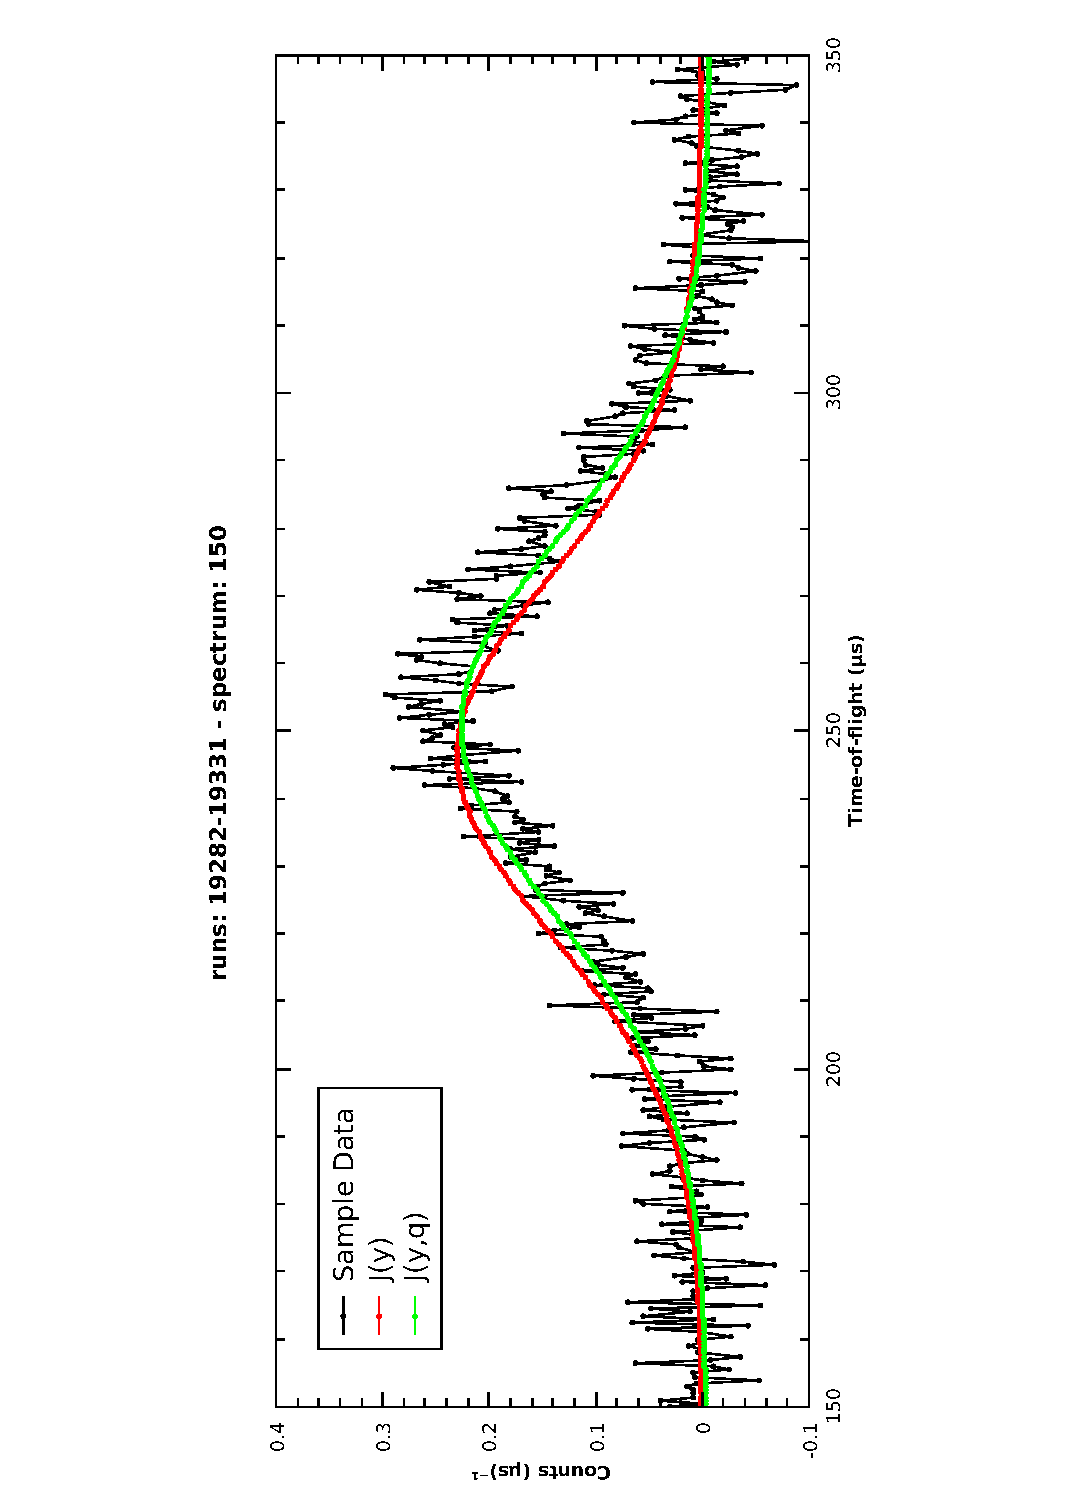
\includegraphics[width=0.68\textwidth]{graphics/mvg_fse_compare.eps}
  \end{turn}
  \vspace{-50pt}
  \caption{Comparison of fit with and without \gls*{FSE} correction}
  \label{fig:mvg_fse_compare}
\end{figure}
\FloatBarrier

This shows a noticeable offset caused by the addition of the correction which
shifts the fitted peak towards the centre of the experimentally measured peak.
The centre of the fitted peak is still slightly towards the low side of the
experimental peak however this offset is reasonable for the quality of the data
and further corrections would only make the function slower to evaluate for only
marginal improvement.

\subsubsection{Effects of integration domain size}
\label{sec:mvg_testing_integration_domain}

The effects of the size of the integration domain are briefly discussed by
Romanelli in which it is summarised that the size of the domain must be at least
$\mathrm{35x35}$, here several additional tests were performed in which the
accuracy of the function relative to the Gram-Charlier profile and execution
times are compared.

The final fitted parameters and execution times for both stages of model fitting
are summarised in table \ref{tab:mvg_integration_compare_params}, only the
parameters relevant to the multivariate Gaussian function are listed (note that
the mass parameter is fixed to 1.0079 for the Hydrogen peak).

\begin{table}[h!]
  \centering
  \begin{tabular}{@{}lllll@{}}
    \toprule
    Domain dimensions    & 8x8     & 32x32    & 64x4     & 256x256 \\
    \midrule
    SigmaX               & 2.49073 & 5.06038  & 8.25955  & 12.2212 \\
    SigmaY               & 11.7155 & 5.06598  & 2.51403  & 2.04771 \\
    SigmaZ               & 3.1926  & 4.3432   & 4.20634  & 4.16945 \\
    Intensity            & 1.20557 & 0.937984 & 0.945023 & 1.18128 \\
    Cost function        & 1.10373 & 1.20871  & 1.20523  & 1.07845 \\
    Initial fit time (s) & 3.8     & 49.3     & 151.4    & 2456.4  \\
    Final fit time (s)   & 6.2     & 34.6     & 152      & 2591    \\
    \bottomrule
  \end{tabular}
  \caption{Comparison of final fitted parameters and execution times for
           different integration domain dimensions}
  \label{tab:mvg_integration_compare_params}
\end{table}
\FloatBarrier

Figure \ref{fig:mvg_integration_compare_1} shows a comparison between the
Gram-Charlier profile (black line) and the four different integration domain
dimensions: $\mathrm{8x8}$ (cyan line), $\mathrm{32x32}$ (green line),
$\mathrm{64x64}$ (blue line) and $\mathrm{256x256}$ (red line).

This plot shows the majority of the fitted time of flight range used in VESUVIO
model fitting, this emphasises the changing shape of the wings of the peak at
$< 200 \mathrm{\mu s}$ and $> 300 \mathrm{\mu s}$.

Note that the peak at approx. $370 \mathrm{\mu s}$ is from a combination of
Carbon and Oxygen, both of which are fitted using the standard isotropic
Gaussian hence will have the same peak shape in all fitted spectra.

\begin{figure}[h!]
  \centering
  \begin{turn}{-90}
    \includegraphics[width=0.75\textwidth]{graphics/mvg_integration_compare_1.eps}
  \end{turn}
  \vspace{-80pt}
  \caption{General comparison of different integration domain dimensions}
  \label{fig:mvg_integration_compare_1}
\end{figure}
\FloatBarrier

Figure \ref{fig:mvg_integration_compare_2} shows the same fitted spectra as
figure \ref{fig:mvg_integration_compare_1} with the plot area focused around the
Hydrogen peak. This provides a good view of the quality of each fit in terms of
its peak centre and shape with respect to the Gram-Charlier profile.

\begin{figure}[h!]
  \centering
  \begin{turn}{-90}
    \includegraphics[width=0.75\textwidth]{graphics/mvg_integration_compare_2.eps}
  \end{turn}
  \vspace{-80pt}
  \caption{Comparison of different integration domain dimensions at Hydrogen
           peak}
  \label{fig:mvg_integration_compare_2}
\end{figure}
\FloatBarrier

Given the lower cost function value is assigned to the domain of size
$\mathrm{256x256}$ this fit is likely to be the best description of the data,
however looking at the plot of each fitted spectrum around the Hydrogen peak in
figure \ref{fig:mvg_integration_compare_2} it can be seen that the
$\mathrm{256x256}$ domain (red line) is one of the furthest from the
Gram-Charlier profile (black line). Ideally the multivariate Gaussian profile
should be a close math to the Gram-Charlier profile. Having said this the final
parameters produced by the fit using the $\mathrm{256x256}$ domain are
somewhat reasonable given the data.

Furthermore the computational cost of this as reflected by the execution time
for both fitting stages makes this improvement in fit quality infeasible for
general use.

Comparatively the $\mathrm{8x8}$ domain which is expected to have a poor fit
quality is fairly close to the much finder $\mathrm{256x256}$ sized domain.

The domains of size $\mathrm{32x32}$ and $\mathrm{64x64}$ both produce a similar
and reasonable fit, however the parameters produced by the $\mathrm{64x64}$
domain are the best description of the data out of all that have been fitted as
part of this test.

As such this was set as the default domain size and is the size used for the
evaluation performed in section \ref{sec:mvg_case_studies}.

\subsubsection{Automated Testing}

The multivariate Gaussian fitting model is tested to the same extent as all
other fitting models for VESUVIO data via a set of unit and system tests that
are run as part of the \gls*{MANTID} continuous integration system.

These tests are mainly designed as simple logical tests to ensure that the
fit function and associated profile in the workflow scripts behave as expected
in terms of the workflow rather than the quality of the fitted data its self.

That being said there is a basic test that the function, when evaluated with a
given set of parameters, gives the correct values. As well as a function that
tests the generation of the $S^{2}$ matrix.

\subsubsection{Informal Testing}
\label{sec:mvg_informal_testing}

Several informal tests were carried out as part of the development process; this
included tests done by myself, the instrument scientist and the developer that
approved the changes to \gls*{MANTID}.

This testing is a good source of a second opinion on the implemented function
both from the scientific and software engineering perspectives.

Having the model tested by the scientist did highlight an issue that had
previously gone unnoticed due to not being directly related to the work being
carried out. As mentioned in section \ref{sec:existing_data_analysis_workflow}
an initial fit is performed to obtain a set of parameters to be used in the
calculation of several corrections, one of which - the multiple scattering
correction - when using parameters form the multivariate Gaussian profile was
giving a largely underestimated correction for the area around the Hydrogen peak
the function was fitting where there is known to be a large multiple scattering
contribution to the measured signal.

Figure \ref{fig:mvg_multiple_scattering_corr} shows the difference is multiple
scattering correction caused by the differing parameters which are in turn
provided in table \ref{tab:mvg_ms_params}.

In this table the function fitting the Hydrogen peak is the first function in
the composite function \texttt{f0}. The values given for the width of the
multivariate Gaussian function are obtained using the following equation which
is used in the workflow script to convert the \texttt{Sigma[X,Y,Z]} parameters
into a single width parameter $\bar{\sigma}$ for the multiple scattering
correction algorithm.

\begin{equation}
  \label{eq:mvg_ms_width}
  \bar{\sigma} =
    \sqrt{\frac{\sigma_{x}^{2} + \sigma_{y}^{2} + \sigma_{z}^{2}}{3}}
\end{equation}

\begin{table}[h!]
  \centering
  \begin{tabular}{lllll}
    \toprule
                  & Gram-Charlier & Error      & Multivariate & Error     \\
    \midrule
    f0.Mass       & 1.0079        & 0          & 1.0079       & 0         \\
    f0.Width      & 4.48946       & 0.122974   & 8.19068      & -         \\
    f0.SigmaX     & -             & -          & 2.96842      & 1.53772   \\
    f0.SigmaY     & -             & -          & 13.4967      & 0.664743  \\
    f0.SigmaZ     & -             & -          & 3.20772      & 1.18797   \\
    f0.Intensity  & 69.1487       & 1.76213    & 0.967407     & 0.216778  \\
    f1.Mass       & 12.011        & 0          & 12.011       & 0         \\
    f1.Width      & 10            & 0          & 10           & 0         \\
    f1.Intensity  & 0.170138      & 1.07746    & 1.41289      & 1.29345   \\
    f2.Mass       & 15.9          & 0          & 15.9         & 0         \\
    f2.Width      & 13            & 0          & 13           & 0         \\
    f2.Intensity  & 5.78972       & 1.05313    & 5.53164      & 1.21508   \\
    f3.A0         & 0.0086126     & 0.00491099 & 0.0200821    & 0.0047604 \\
    f3.A1         & -116.651      & 40.4553    & -274.6       & 45.23     \\
    f3.A2         & 201.274       & 65400.6    & 462892       & 76824.8   \\
    Cost Function & 1.0404        & 0          & 1.21149      & 0         \\
    \bottomrule
  \end{tabular}
  \caption{Fitted parameters used for multiple scattering calculation}
  \label{tab:mvg_ms_params}
\end{table}
\FloatBarrier

As shown in table \ref{tab:mvg_ms_params} the calculated with of the
multivariate Gaussian profile is almost double that of the Gram-Charlier
profile, however it is much more likely that the significantly lower intensity
is the cause of the difference in multiple scattering calculation.

The reduced intensity is effectively removing the relative contribution of the
Hydrogen peak to the multiple scattering in the sample, hence why the
contributions of other masses are increased beyond their contributions when
using the parameters from the Gram-Charlier profile.

\begin{figure}[h!]
  \centering
  \begin{turn}{-90}
    \includegraphics[width=0.7\textwidth]{graphics/mvg_multiple_scattering_corr.eps}
  \end{turn}
  \vspace{-80pt}
  \caption{Comparison of multiple scattering corrections}
  \label{fig:mvg_multiple_scattering_corr}
\end{figure}
\FloatBarrier

Although not demonstrated the same effects are seen when comparing with the
standard Gaussian profile.

\section{Bayesian model selection}
\label{sec:bayesian_analysis_routines}

The second objective is to develop and integrate a model selection algorithm
that given a set of raw time of flight data from the instrument can obtain a
fitting model that best describes the data, this will be used to aid analysis in
cases where the sample contains unexpected impurities that contribute to
additional mass peaks or when the composition of the sample is unknown.

\subsection{Background}
\label{sec:bayes_background}

The model selection algorithm will use Bayesian model selection to select the
most likely model form a set of hypothesis, this has been chosen due to the wide
use of this methodology in various other neutron scattering data analysis
workflows.

Probability theory gives the two basic rules: the sum rule; given the
probability of $x$ being true we can derive the probability of $x$ being false
and the product rule; given the probability of $x$ being true and the
probability of $y$ being true we can derive the probability of both $x$ and $y$
being true, given in equations \ref{eq:prob_sum_rule} and
\ref{eq:prob_product_rule} respectively.

\begin{equation}
  \label{eq:prob_sum_rule}
  P(x | I) + P(\bar{x} | I) = 1
\end{equation}

\begin{equation}
  \label{eq:prob_product_rule}
  P(x, y | I) = P(x | y, I) \times P(y | I)
\end{equation}

where; $|$ denotes a "given that" relationship between two events, $\bar{x}$
denotes the case where $x$ is false and $I$ is background information that could
affect the probability of either $x$ or $y$.

Given experimental data the measurable probability is that of the data given a
hypothesis $P(D|H)$, however in data analysis the desirable probability to
measure is the probability of a hypothesis given the experimental data $P(H|D)$.

\begin{equation}
  \label{eq:bayes_theorem}
  P(x | y, I) = \frac{P(y | x, I) \times P(x | I)}{P(y | I)}
\end{equation}

Using Bayes' theorem given in equation \ref{eq:bayes_theorem} it is possible to
effectively swap the dependency order of the given that relation between the
hypothesis and data. \cite{Sivia1993}

Take for example two unique hypotheses $A$ and $B$, in order to determine which
best describes data $D$ the ratio of their probabilities given the data can be
calculated as

\begin{align}
  \label{eq:bayes_example_1}
              posterior &= prior \times Bayes \: factor \\
  \frac{P(A|D)}{P(B|D)} &= \frac{P(A)}{P(B)} \times \frac{P(D|A)}{P(D|B)}
\end{align}

where the prior ratio is used to define the probability ratio of the two
hypotheses based on prior knowledge, i.e. disregarding the data $D$.

This model works when both $A$ and $B$ are simple hypotheses that do not rely on
fitted parameters, however assuming hypothesis $B$ required an additional
parameter to define the model the value of this parameter must be considered in
the calculation of the probability ratio.

\begin{align}
  \label{eq:bayes_example_2}
  posterior &= prior \times Bayes \: factor \times Ockham factor \\
  \frac{P(A|D)}{P(B|D)} &=
    \frac{P(A)}{P(B)} \times
    \frac{P(D|A)}{P(D|\lambda_{0}, B)} \times
    \frac{\lambda_{max} - \lambda_{min}}{\delta\lambda}
\end{align}

Equation \ref{eq:bayes_example_2} \cite{Sivia1993} shows how a fitted parameter
$\lambda$ can be integrated into the model selection. In this case the so called
"Ockham factor" is used to penalise hypothesis $B$ for its additional fitted
parameter, this follows the general desire for the best model to be the one
which best describes the data with the fewest parameters.

Note that the parameters limits $\lambda_{min}$ and $\lambda_{max}$ must be
chosen appropriately, an obvious general case may be to set them to infinity
however this causes an infinite penalty to be applied for the addition of a
parameter. Typically enough is known about the domain of the problem to allow a
sensible selection of these limits.

Most curve fitting in \gls*{MANTID} uses the $\chi^{2}$ cost function as defined
by equation \ref{eq:chi_2}. Typically the $\chi^{2}$ is divided by the number of
free fitting parameters.

\begin{equation}
  \label{eq:chi_2}
  \chi^{2} = \sum_{i=1}^{N} \left(\frac{D_{i} - f(D_{i}, M)}{\sigma_{i}}\right)^{2}
\end{equation}

where; $N$ is the number of data points, $D_{i}$ is the $i$th measured/sample
data point, $f()$ is a function defining the model being fitted, $M$ are
parameters defining the model and $\sigma_{i}$ is the standard error of the
$i$th data point.

One issue with the $\chi^{2}$ cost function is that it has a large dependence on
the shape of the $\chi^{2}$ distribution \cite{Monserrat2015}, for example if no
local minima are found when searching for the global minimum.

The Fitting Algorithm for Bayesian Analysis of DAta (FABADA) provides a fitting
methodology that does not depend on the shape of the cost function or relations
between fitting parameters. This algorithm provides a probability distribution
function for all fitted parameters as well as the cost function, which through
inspection of can be used to create a Bayesian model selection scheme.

The \gls*{FABADA} algorithm is a Markov Chain Monte Carlo algorithm that
operates by randomly changing a fitting parameter and accepting the change if it
causes a decrease in the value of the cost function. There is also a chance
that an increase in the cost function value will be allowed, the probability of
which is given in the equation \cite{Monserrat2015}

\begin{equation}
  \frac{P(H(P_{i}^{new}) | D)}{P(H(P_{i}^{old})|D)} =
    exp\left(-\frac{\chi^{2}_{new} - \chi^{2}_{old}}{2}\right)
\end{equation}

where; $P(H|D)$ is the probability of the hypothesis being true given the
measured data, $H(P_{i})$ is the hypothesis described by parameter set $P_{i}$.

It is this property that allows the \gls*{FABADA} algorithm to "jump" over
obstacles in the shape of the cost function that may cause traditional
Levenberg-Marquardt methods to converge to a non-optimal fit.

One issue of this method is the number of steps in parameter value required to
converge to the optimal solution, to address this the algorithm adds a bias to
the changes applied to each parameter such that parameters who's changes are
infrequently accepted are assigned larger steps in an attempt to invoke a larger
step in the cost function. The opposite of this process happens for parameters
with frequently accepted changes.

Fitting is complete when all parameters have converged, this is defined as the
point at which the probabilities of each parameter have been accepted with equal
probability.

\subsection{Implementation}
\label{sec:bayes_implementation}

The model selection algorithm will be implemented as a new workflow algorithm
within \gls*{MANTID} leveraging already implemented peak finding and fitting
routines.

In this implementation the "model" is described as a composition of fitting
functions that describe the data, typically this is one Compton profile per mass
(where multiple masses can contribute to the same peak) and one background
function which is usually a polynomial of order 2.

In \gls*{MANTID} a model is composed of:

\begin{itemize}
  \item
    A fit function string which defines the functions being fit and their
    initial parameters

  \item
    A ties string which defines values which certain parameters are fixed to,
    this can be either a fixed value of another parameter.

  \item
    A constraints string which defines upper and/or lower constraints for he
    value of certain parameters
\end{itemize}

An example of a typical model for the VESUVIO data analysis workflow for a
sample containing Hydrogen, Oxygen and Caesium in an Aluminium container is as
follows:

\begin{description}
  \item[Function] \hfill \\
    \texttt{
    composite=CompositeFunction,NumDeriv=1;\\
    name=GramCharlierComptonProfile,Mass=1.007900,HermiteCoeffs=1 0 0,Width=4.480264,\\
    FSECoeff=0.528532,C\_0=12.239281;\\
    name=GaussianComptonProfile,Mass=16.000000,Width=10.000000,Intensity=2.829303;\\
    name=GaussianComptonProfile,Mass=27.000000,Width=13.000000,Intensity=0.392174;\\
    name=GaussianComptonProfile,Mass=133.000000,Width=30.000000,Intensity=0.707326;\\
    name=Polynomial,n=2,A0=-0.003896,A1=5.387158,A2=1.003049
    }

  \item[Ties] \hfill \\
    \texttt{
      f0.Mass=1.007900,\\
      f0.FSECoeff=f0.Width*sqrt(2)/12,\\
      f1.Mass=16.000000,\\
      f1.Width=10.000000,\\
      f2.Mass=27.000000,\\
      f2.Width=13.000000,\\
      f3.Mass=133.000000,\\
      f3.Width=30.000000
    }

  \item[Constraints] \hfill \\
    \texttt{
      2.000000 < f0.Width < 7.000000,\\
      f0.C\_0 > 0.0,\\
      f1.Intensity > 0.0,\\
      f2.Intensity > 0.0,\\
      f3.Intensity > 0.0
    }
\end{description}

The fitted results of this model are shown in figure \ref{fig:example_model},
the Hydrogen peak can be seen around the $200 \mu s$ to $300 \mu s$ time of
flight region and the single peak for all higher masses around $380 \mu s$ to
$400 \mu s$.

\begin{figure}[h!]
  \centering
  \begin{turn}{-90}
    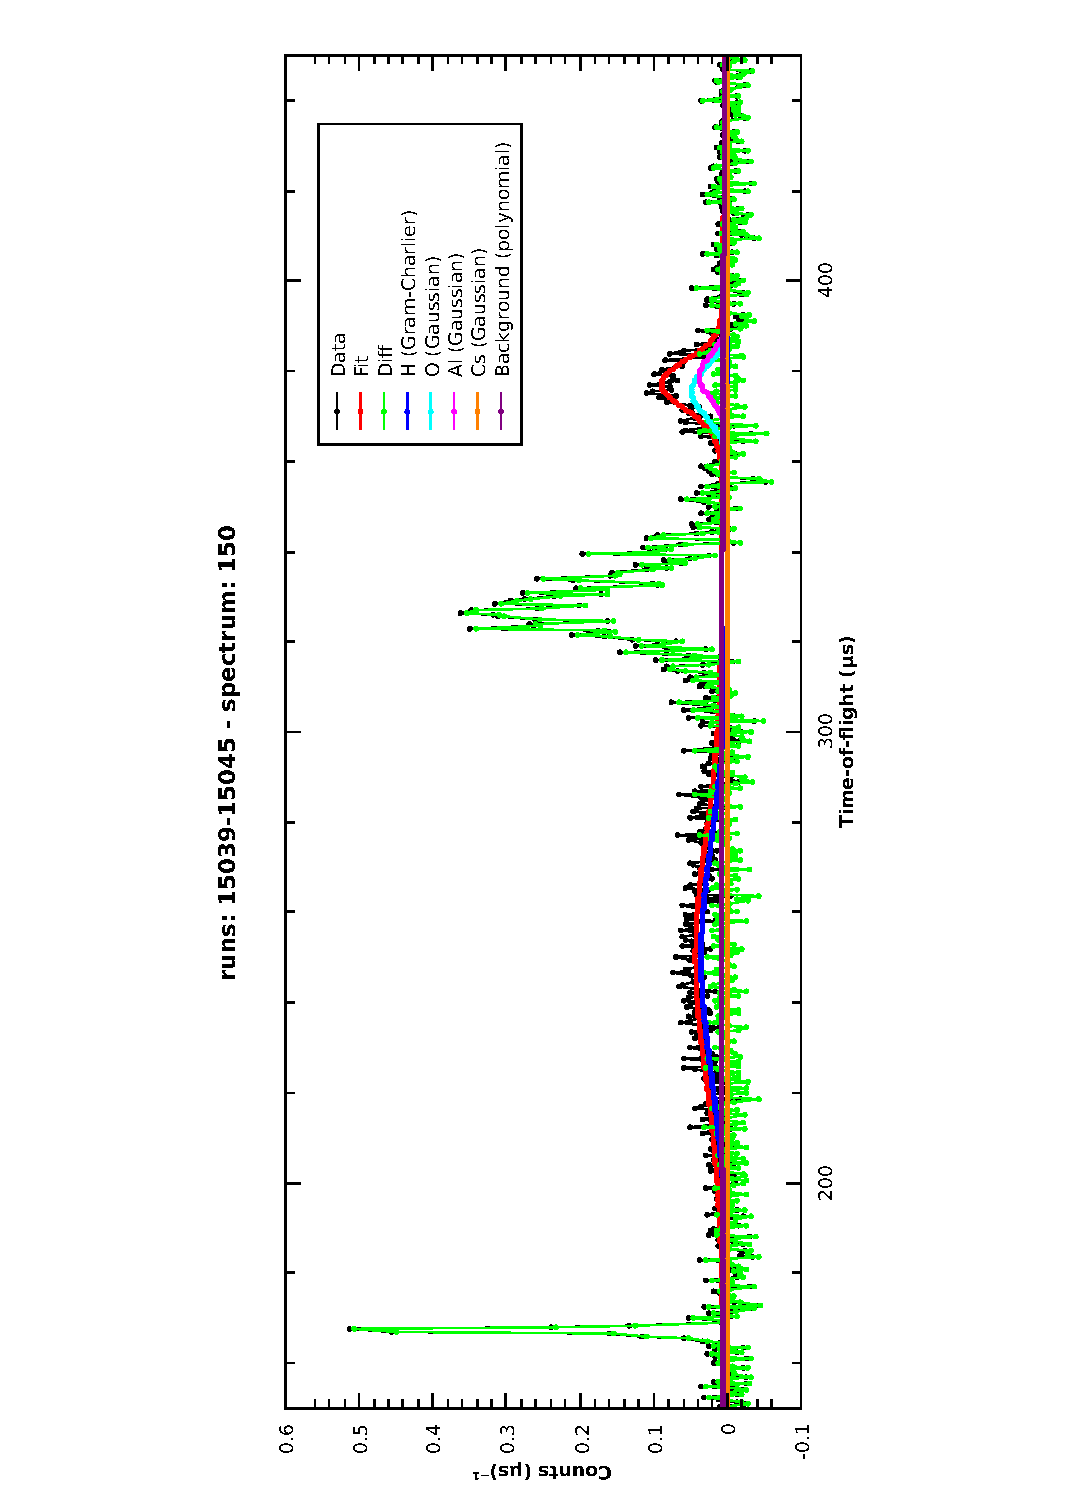
\includegraphics[width=0.6\textwidth]{graphics/exmaple_model.eps}
  \end{turn}
  \vspace{-50pt}
  \caption{Example fitting model}
  \label{fig:example_model}
\end{figure}
\FloatBarrier

The general workflow for the new algorithm is described by figure
\ref{fig:model_sel_workflow}.

\begin{figure}[h!]
  \centering
  \includegraphics[width=0.3\textwidth]{out/model_selection_workflow.1}
  \caption{Model selection algorithm workflow}
  \label{fig:model_sel_workflow}
\end{figure}
\FloatBarrier

In the case of this implementation a model as described above is a single
hypothesis in the context of the Bayesian model selection.

The first step is to load the sample data, this uses the same implementation of
the data loading step as is used in the existing VESUVIO workflow described in
section \ref{sec:existing_data_analysis_workflow}.

The next step is to use the \gls*{MANTID} peak finding algorithm
\texttt{FindPeaks} to search for peaks in all spectra of the loaded data, this
provides an initial guess as to the locations of mass peaks in the measured
data. This peak finding algorithm operates by fitting a Gaussian peak with a
background to the specified input range \cite{Mariscotti1967}, the search can be
refined by providing additional information about the position and nature of the
peak however at this stage no such information is provided.

This list of found peaks is then used as a peak position estimate in order to
find a reasonable accurate peak position and shape for the relevant peak on each
spectrum.

After this operation a list of reasonably accurate peaks for each spectrum will
have been generated, these are then used to generate a list of models for the
Bayesian model selection. This is done by assuming that each detected peak can
have between 0 and 4 masses contribute to it (this is a fixed value at the
moment but should be exposed to the user as a property for the algorithm) then
creating a model with each permutation of number of masses for each peak.

Take, for example the following peaks having been found in a spectrum:

\begin{table}[h!]
  \centering
  \begin{tabular}{@{}ll@{}}
    \toprule
    Position    & Width \\
    \midrule
    $250 \mu s$ & 15    \\
    $370 \mu s$ & 8     \\
    \bottomrule
  \end{tabular}
  \caption{Example found peaks}
  \label{tab:ba_example_peaks}
\end{table}
\FloatBarrier

The following 25 models would be created:

\begin{table}[h1]
  \centering
  \begin{tabular}{@{}lll@{}}
    \toprule
    Model & Peaks under $250 \mu s$ & Peaks under $370 \mu s$ \\
    \midrule
    0     & 0                       & 0                       \\
    1     & 1                       & 0                       \\
    2     & 2                       & 0                       \\
    3     & 3                       & 0                       \\
    4     & 4                       & 0                       \\
    5     & 0                       & 1                       \\
    6     & 1                       & 1                       \\
    7     & 2                       & 1                       \\
    8     & 3                       & 1                       \\
    9     & 4                       & 1                       \\
    10    & 0                       & 2                       \\
    11    & 1                       & 2                       \\
    12    & 2                       & 2                       \\
    13    & 3                       & 2                       \\
    14    & 4                       & 2                       \\
    15    & 0                       & 3                       \\
    16    & 1                       & 3                       \\
    17    & 2                       & 3                       \\
    18    & 3                       & 3                       \\
    19    & 4                       & 3                       \\
    20    & 0                       & 4                       \\
    21    & 1                       & 4                       \\
    22    & 2                       & 4                       \\
    23    & 3                       & 4                       \\
    24    & 4                       & 4                       \\
    \bottomrule
  \end{tabular}
  \caption{Example models}
  \label{tab:ba_example_models}
\end{table}
\FloatBarrier

In the models generated by the algorithm only the standard isotropic Gaussian
function is used and has its mass parameter constrained based on the width of
the peak found in the peak finding stage.

The limits of the mass constraint are obtained by taking the limits in time of
flight which are calculated by taking the peak position plus/minus the
\gls*{HWHM}, these limits in time of flight are then converted into limits in
atomic mass using equations \ref{eq:ba_toftomass_1} and \ref{eq:ba_toftomass_2}.

\begin{equation}
  \label{eq:ba_toftomass_1}
  tof = \frac{L_{0}r_{t} + L_{1}}{v_{0}}
\end{equation}

where; $L_{0}$ is the length of the primary flight path (form moderator to
sample), $L_{1}$ is the length of the secondary flight path (from sample to
detector), $v_{0}$ is the final neutron velocity and $r_{t}$ is given by
equation \ref{eq:ba_toftomass_2}.

\begin{equation}
  \label{eq:ba_toftomass_2}
  r_{t} =
    \frac{cos\theta + \sqrt{\frac{m}{m_{n}}^{2}-sin^{2}\theta}}
         {\frac{m}{m_{n}} + 1}
\end{equation}

where; $\theta$ is the scattering angle, $m$ is the mass of the atomic mass of
the stuck nucleus and $m_{n}$ is the atomic mass of the neutron.

The following fitting is then performed per generated model per spectrum in the
sample data.

Additional constrains on the model include the requirement for both the
intensity and width parameters to be positive non zero values and that masses
fitted by each Gaussian function must be unique to prevent the same mass being
fitted by multiple functions.

These models are then fitted to each spectrum using the standard
Levenberg-Marquardt algorithm in order to obtain a reasonable set of starting
parameters for the fit using the \gls*{FABADA} minimiser which is known to
require good parameters when a fit is performed over a large number of degrees
of freedom. This is also the reason parameters are constrained whenever possible
in order to narrow the search space as much as it can be.

Once a set of starting parameters is derived the model is then fitted using the
\gls*{FABADA} minimiser to obtain a refined set of parameters and their
probability, the probabilities of each model are then compared and the most
likely selected as the best model.

\subsection{Testing}
\label{sec:bayes_testing}

\subsubsection{Automated Testing}

As the model selection algorithms is yet to be functional to the full
satisfaction of the instrument scientist no automated tests have been written
for it as of yet.

\subsubsection{Informal Testing}
\label{sec:bayes_informal_testing}

Throughout the implementation of the algorithm several stages of informal
testing were performed to asses the accuracy and reliability of independent
stages of the algorithm (which were in turn typically separate algorithms
already implemented in \gls*{MANTID}).

One of the main examples of this was in the output generated by the
\texttt{FindPeaks} algorithm which was used to perform the initial significant
peak finding to search for peaks that could correspond to a mass peak.

The most significant issue raised by the use of this algorithm is the wide range
of results given by the algorithm when executed with different data sets; some
of which give a reasonable estimation of the location of peaks, some assign
peaks to noise while missing larger more visually obvious peaks and some fail to
find any peaks.

Several examples of common problems are shown with four samples; Iodobenzoic
acid (\chem{C_{7}H_{5}IO_{2}}), Polycrystalline zirconium-beryllium
(\chem{Zr_{40}Be_{20}}), Squaric acid (\chem{C_{4}H_{2}O_{4}}) and Graphite
(\chem{C}). All samples are in Aluminium containers with the exception of
Graphite which is in a Tin container.

Figure \ref{fig:peakfind_iodobenzoic_acid} shows the raw time of flight spectrum
for a sample of Iodobenzoic acid in an Aluminium container, here true peaks are
observed at around $200 \mu s$ to $300 \mu s$ for the Hydrogen peak and around
$350 \mu s$ to $420 \mu s$ for heavier masses.

\begin{figure}[h!]
  \centering
  \begin{turn}{-90}
    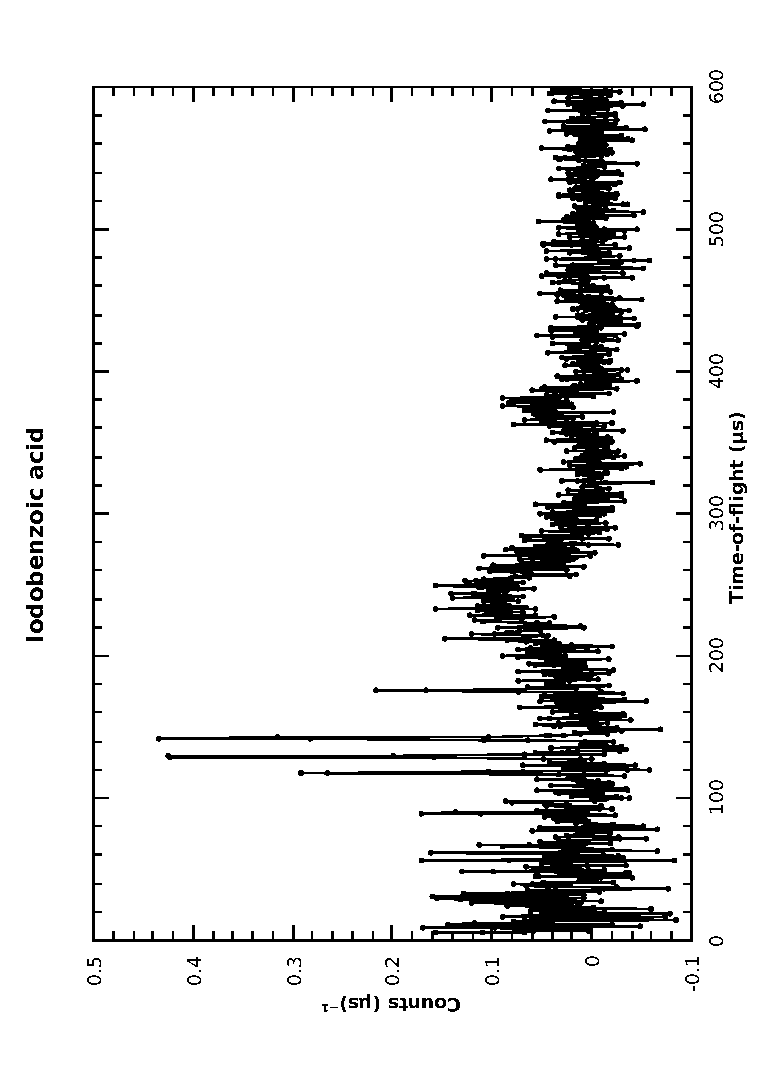
\includegraphics[width=0.4\textwidth]{graphics/peakfind_iodobenzoic_acid.eps}
  \end{turn}
  \caption{Raw spectrum of Iodobenzoic acid sample}
  \label{fig:peakfind_iodobenzoic_acid}
\end{figure}
\FloatBarrier

Table \ref{tab:peakfind_iodobenzoic_acid} shows the results of the peak finding
algorithm. In this case no true peaks were found by the algorithm, instead the
two tallest peaks in the spectrum caused by noise were reported as the
significant peaks in the sample.

\begin{table}[h!]
  \centering
  \begin{tabular}{@{}lll@{}}
    \toprule
    Position ($\mu s$) & Width   & Height \\
    \midrule
    117.848            & 1.07304 & 0.304676 \\
    129.286            & 1.33195 & 0.453472 \\
    \bottomrule
  \end{tabular}
  \caption{Peak finding results for Iodobenzoic acid}
  \label{tab:peakfind_iodobenzoic_acid}
\end{table}
\FloatBarrier

The polycrystalline zirconium-beryllium sample (figure
\ref{fig:peakfind_pczrbe}) is an example of where the results of peak finding
contain both true and spurious peaks.

\begin{figure}[h!]
  \centering
  \begin{turn}{-90}
    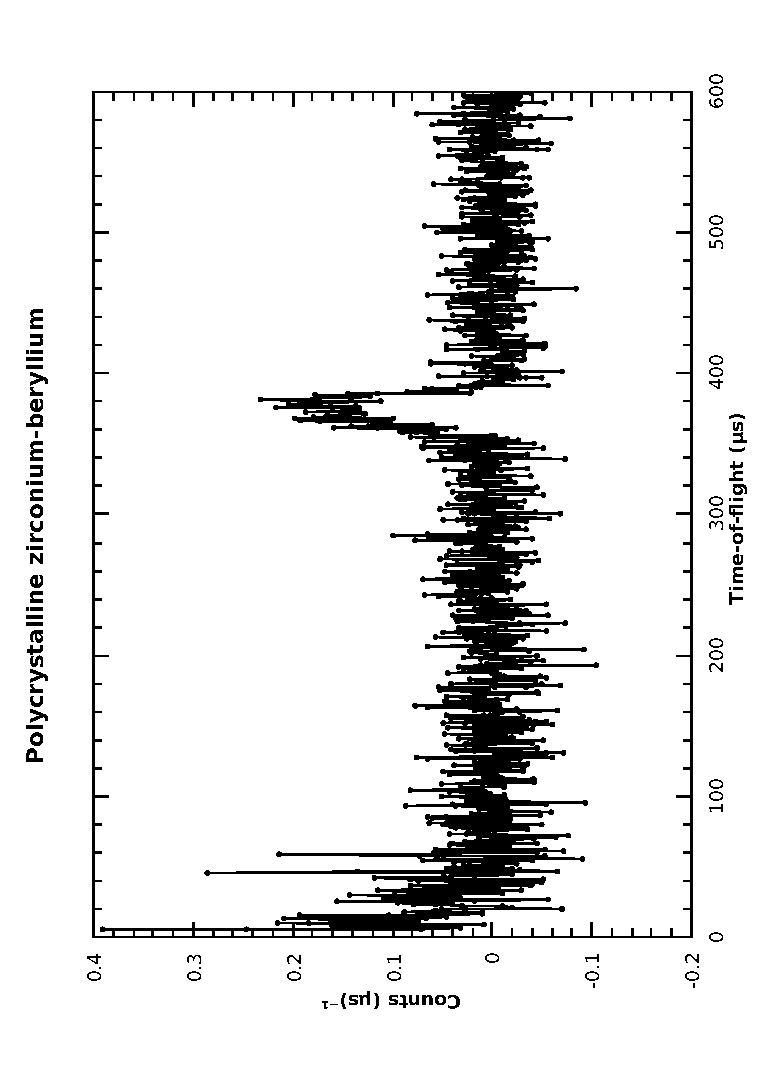
\includegraphics[width=0.4\textwidth]{graphics/peakfind_pczrbe.eps}
  \end{turn}
  \caption{Raw spectrum of Polycrystalline zirconium-beryllium sample}
  \label{fig:peakfind_pczrbe}
\end{figure}
\FloatBarrier

In this case the peak caused by the masses known to be present in the sample is
detected correctly (the peak at around $374 \mu s$) however an additional peak has
been found in noise at around $285 \mu s$.

\begin{table}[h!]
  \centering
  \begin{tabular}{@{}lll@{}}
    \toprule
    Position ($\mu s$) & Width   & Height    \\
    \midrule
    285.225            & 1.63995 & 0.0685314 \\
    374.626            & 21.1158 & 0.129163  \\
    \bottomrule
  \end{tabular}
  \caption{Peak finding results for Polycrystalline zirconium-beryllium}
  \label{tab:peakfind_pczrbe}
\end{table}
\FloatBarrier

In the case of the Squaric acid sample (figure \ref{fig:peakfind_sq_acid}) the
issue is the lack of detection of a true peak, in this case the Hydrogen peak
between $180 \mu s$ and $310 \mu s$. This is the most acceptable case of the
peak finding algorithm failing to identify all peaks successfully and is partly
to be expected by the significantly larger width of the Hydrogen peak.

\begin{figure}[h!]
  \centering
  \begin{turn}{-90}
    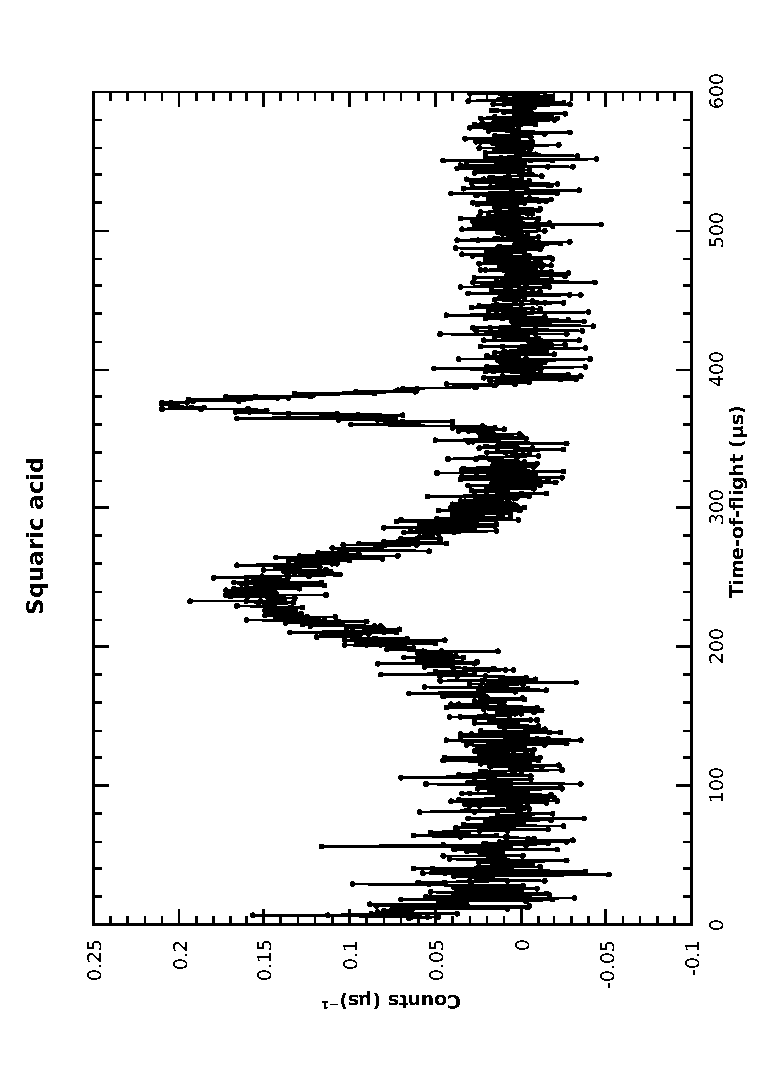
\includegraphics[width=0.4\textwidth]{graphics/peakfind_squaric_acid.eps}
  \end{turn}
  \caption{Raw spectrum of Squaric acid sample}
  \label{fig:peakfind_sq_acid}
\end{figure}
\FloatBarrier

The peak contributed to by heavier masses ($330 \mu s$ to $400 \mu s$) has been
identified correctly in this case, as is shown in table
\ref{tab:peakfind_sq_acid}.

\begin{table}[h!]
  \centering
  \begin{tabular}{@{}lll@{}}
    \toprule
    Position ($\mu s$) & Width   & Height   \\
    \midrule
    374.164            & 17.4555 & 0.191177 \\
    \bottomrule
  \end{tabular}
  \caption{Peak finding results for Squaric acid}
  \label{tab:peakfind_sq_acid}
\end{table}
\FloatBarrier

The peak finding algorithm failed to find any significant peaks in the Graphite
sample shown in figure \ref{fig:peakfind_graphite}. The two most likely causes
of this is the relative intensity of the true peak to the background noise and
the non-Gaussian distribution of the peak, both in the asymmetry and overly
steep falling edge of the peak.

\begin{figure}[h!]
  \centering
  \begin{turn}{-90}
    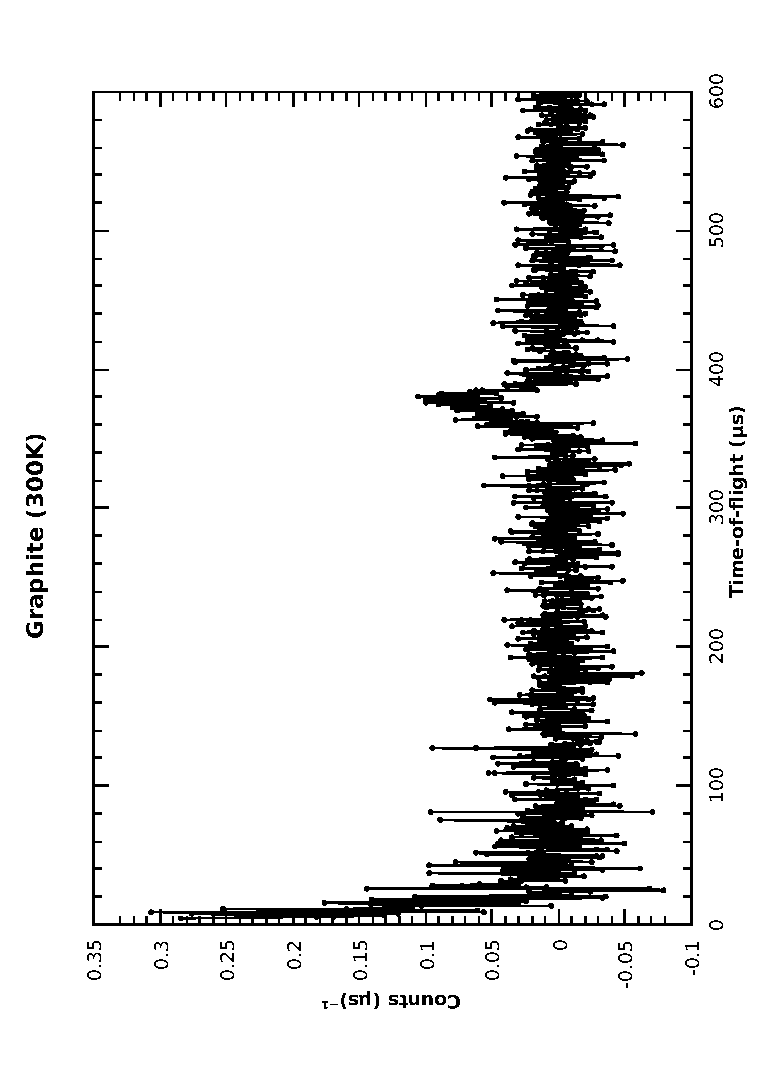
\includegraphics[width=0.4\textwidth]{graphics/peakfind_graphite.eps}
  \end{turn}
  \caption{Raw spectrum of Graphite sample at 300K}
  \label{fig:peakfind_graphite}
\end{figure}
\FloatBarrier

Typically this issue can be resolved by changing the parameters to the
\texttt{FindPeaks} algorithm, most notable the \textit{FWHM} and
\textit{Tolerance} parameters.

The wide variation of peak widths can often mean fitting a single Gaussian width
(determined by the \texttt{FWHM} parameter) can cause only a subset of true
peaks to be found while possibly selecting false peaks in the noise, in the
current peak finding solution this is a non-trivial problem to overcome without
requiring a new peak finding implementation.

An additional problem is setting a reasonable tolerance for the required
acceptance of peaks, this tolerance value is used in the implementation of the
peak finding algorithm as described by Mariscotti \cite{Mariscotti1967} where a
lower value gives rise to stricter peak selection.

Having this value incorrectly set can cause either true peaks to be missed if
the value is too low or additional peaks being found in noise if the value is
too high.

Another area that underwent ongoing manual testing was the quality of the
models generated by an initial fit using the Levenberg-Marquardt algorithm.
Typically this worked as expected where a model with a rough estimation of a
peak position would have its mass fitted to be close to the mass that
contributed to the majority of the peak.

However one significant issue with the initial fitting routine is that when
fitting a model in which there are several profiles that are attempting to fit a
single peak which is defined by less than the number of profiles (for instance
attempting to fit 4 masses to a peak that was only contributed to by 2) the
masses of multiple profiles tended to converge on the same mass.

This was a significant issue as it artificially increased the suitability of
more complex models by obtaining parameters that give a value to the cost
function $\chi^{2}$ that is only marginally worse than that of a simpler model.

While the $\chi^{2}$ of the initial fit is not inspected as the only purpose of
this algorithm is to find a likely set of models this issue causes a reduction
in the number of possible models due to lack of exploration of the full search
space of the mass parameter, possibly excluding a correct mass from the
Bayesian model selection that follows on from this initial fitting.

A solution to that above two issues can be to allow the user to modify the range
of Gaussian widths and tolerances over which the \texttt{FindPeaks} algorithm is
executed, however the need for the user to run the algorithm in order to look at
the results and possibly have to change input parameters and execute the
algorithm a further time until the results are reasonable somewhat negates the
point of using this algorithm in the first place. Having said that the peak
finding is a relatively computationally cheap operation compared to the full
VESUVIO analysis routine so this process of manually modifying parameters to
obtain good results at this stage is not as time consuming as doing the same
with the full data analysis workflow.

\section{Evaluation though Case Studies}
\label{sec:evaluation_through_case_studies}

Several case studies have been used to provide testing of the results of the new
features implemented as part of this project.

This method of testing has the advantage that it is testing the routines in the
same way in which they are intended to be used, this is not usually possible
through unit testing and is due to build server time constraints usually limited
to a small range of sample data when running as an automated system test.

\subsection{Fitting Hydrogen peaks with a multivariate Gaussian}
\label{sec:mvg_case_studies}

One of the most common use cases for a function that fits an anisotropic mass
peak (i.e. the Gram-Charlier profile or multivariate Gaussian profile) is in
fitting Hydrogen peaks.

These case studies will focus on the comparison of the existing Gram-Charlier
profile and new multivariate Gaussian profile in the quality of the description
of the sample data. The mean kinetic energy along each axis will also be
calculated using equation \ref{eq:mvg_sigma_to_energy} and compared with
published data.

Two well studied hydrogenous samples will be used; water at 300K and ice at
260K.

\subsubsection{Water}

The fitted curves for for both the Gram-Charlier profile and multivariate
Gaussian profile are given in figures \ref{fig:gc_water_fit} and
\ref{fig:mvg_water_fit} respectively.

The Gram-Charlier fit is visually a very good fit of the data, shown by the mass
profile for the Hydrogen peak (blue line) closely following that of the sample
data (black line).

\begin{figure}[h!]
  \centering
  \vspace{-60pt}
  \begin{turn}{-90}
    \includegraphics[width=0.68\textwidth]{graphics/cs_water_gc.eps}
  \end{turn}
  \vspace{-60pt}
  \caption{Fitting results for water sample using Gram-Charlier}
  \label{fig:gc_water_fit}
\end{figure}
\FloatBarrier

In the case of the fit using the multivariate Gaussian the fit is of a
noticeably lower quality. The peak centre can be seen to be shifted to the left
slightly giving a "kink" to the greed difference curve, this can be indicative
of an understated final state effects correction.

Another possibility is the lack of exploration of the full parameter space. This
can be an issue with fit functions with a high degree of freedom using the
Levenberg-Marquardt optimisation function in that a premature minima may be
reached in the cost function which is not the global minimum.

\begin{figure}[h!]
  \centering
  \vspace{-60pt}
  \begin{turn}{-90}
    \includegraphics[width=0.68\textwidth]{graphics/cs_water_mvg.eps}
  \end{turn}
  \vspace{-60pt}
  \caption{Fitting results for water sample using multivariate Gaussian}
  \label{fig:mvg_water_fit}
\end{figure}
\FloatBarrier

Parameters for both functions are given by tables \ref{tab:gc_water_params} and
\ref{tab:mvg_water_params} respectively.

\begin{table}[h!]
  \centering
  \begin{tabular}{lll}
    \toprule
    Parameter     & Value     & Error      \\
    \midrule
    f0.Mass       & 1.0079    & 0          \\
    f0.Width      & 5         & 0.126964   \\
    f0.FSECoeff   & 0.5892556 & 0          \\
    f0.C\_0       & 109.027   & 2.74958    \\
    f1.Mass       & 12.011    & 0          \\
    f1.Width      & 10        & 0          \\
    f1.Intensity  & 0         & 1.26891    \\
    f2.Mass       & 15.9      & 0          \\
    f2.Width      & 13        & 0          \\
    f2.Intensity  & 5.82717   & 1.24073    \\
    f3.A0         & -0.004548 & 0.00589503 \\
    f3.A1         & 8.367988  & 48.387     \\
    f3.A2         & 1.004511  & 79719.6    \\
    Cost Function & 1.149798  & 0          \\
    \bottomrule
  \end{tabular}
  \caption{Fitted parameters for water sample using Gram-Charlier}
  \label{tab:gc_water_params}
\end{table}
\FloatBarrier

Note that in the case of the fit using the Gram-Charlier profile the parameter
errors are relatively low given the value of each parameter, this is reflective
of the good quality of the fit.

\begin{table}[h!]
  \centering
  \begin{tabular}{lll}
    \toprule
    Parameter     & Value     & Error     \\
    \midrule
    f0.Mass       & 1.0079    & 0         \\
    f0.SigmaX     & 3.0069848 & 9.52070   \\
    f0.SigmaY     & 3.5111716 & 16.91488  \\
    f0.SigmaZ     & 4.1116870 & 3.414547  \\
    f0.Intensity  & 0.8536424 & 0.83102   \\
    f1.Mass       & 12.011    & 0         \\
    f1.Width      & 10        & 0         \\
    f1.Intensity  & 0.0216973 & 1.278684  \\
    f2.Mass       & 15.9      & 0         \\
    f2.Width      & 13        & 0         \\
    f2.Intensity  & 3.35907   & 1.24844   \\
    f3.A0         & -0.01038  & 0.005909  \\
    f3.A1         & 4.224282  & 46.1621   \\
    f3.A2         & 2595.102  & 75832.87  \\
    Cost Function & 1.68549   & 0         \\
    \bottomrule
  \end{tabular}
  \caption{Fitted parameters for water sample using multivariate Gaussian}
  \label{tab:mvg_water_params}
\end{table}
\FloatBarrier

In the case of the multivariate Gaussian the parameter errors are noticeably
larger, particularly for the $\sigma_{\alpha}$ parameters of the multivariate
Gaussian profile.

Table \ref{tab:mvg_ke_water} shows a companion between the mean kinetic energies
calculated for the sample analysed above and a similar water sample (at 285K)
analysed by Romanelli.

\begin{table}[h!]
  \centering
  \begin{tabular}{lll}
    \toprule
    Parameter                 & Multivariate Gaussian & Romanelli \cite{Romanelli2015} \\
    \midrule
    $\left<E_{K}\right>_{x}$  & 46.25                 & 18.3                           \\
    $\left<E_{K}\right>_{y}$  & 63.05                 & 51.8                           \\
    $\left<E_{K}\right>_{z}$  & 86.46                 & 83.8                           \\
    \bottomrule
  \end{tabular}
  \caption{Comparison of mean kinetic energies ($\mathrm{meV}$)}
  \label{tab:mvg_ke_water}
\end{table}
\FloatBarrier

The results of my implementation give similar results to that of Romanelli's
previous analysis, there are obvious deviations from is results however given
the errors on the parameters produced by my results this is certainly expected.

\subsubsection{Ice}

Fitted curves for the same profile fitting data from a sample of ice are shown
for the Gram-Charlier profile and multivariate Gaussian profile in figures
\ref{fig:gc_ice_fit} and \ref{fig:mvg_ice_fit} respectively.

As before the Gram-Charlier profile is a very good fit given the noise in the
sample data. Some small fluctuations in the difference curve (shown in green)
can be seen under the Hydrogen peak.

\begin{figure}[h!]
  \centering
  \vspace{-60pt}
  \begin{turn}{-90}
    \includegraphics[width=0.68\textwidth]{graphics/cs_ice_gc.eps}
  \end{turn}
  \vspace{-60pt}
  \caption{Fitting results for ice sample using Gram-Charlier}
  \label{fig:gc_ice_fit}
\end{figure}
\FloatBarrier

Similarly in the fit using the multivariate Gaussian profile, the Hydrogen peak
is fitted reasonably well. There are two noticeable peaks in the difference
curve at either side of the Hydrogen peak, this is due to convergence on bad
fitting parameters.

\begin{figure}[h!]
  \centering
  \vspace{-60pt}
  \begin{turn}{-90}
    \includegraphics[width=0.68\textwidth]{graphics/cs_ice_mvg.eps}
  \end{turn}
  \vspace{-60pt}
  \caption{Fitting results for ice sample using multivariate Gaussian}
  \label{fig:mvg_ice_fit}
\end{figure}
\FloatBarrier

The parameters for both fitting models are shown in tables
\ref{tab:gc_ice_params}, for the Gram-Charlier profile and
\ref{tab:mvg_ice_params} for the multivariate Gaussian.

\begin{table}[h!]
  \centering
  \begin{tabular}{lll}
    \toprule
    Parameter     & Value        & Error     \\
    \midrule
    f0.Mass       & 1.0079       & 0         \\
    f0.Width      & 4.61202317   & 0.36917   \\
    f0.FSECoeff   & 0.543532     & 0         \\
    f0.C\_0       & 115.3064     & 8.69815   \\
    f1.Mass       & 12.011       & 0         \\
    f1.Width      & 10           & 0         \\
    f1.Intensity  & -7.05674e-07 & 0.0223604 \\
    f2.Mass       & 15.9         & 0         \\
    f2.Width      & 13           & 0         \\
    f2.Intensity  & 5.689151     & 1.56584   \\
    f3.A0         & -0.0068479   & 0.0199176 \\
    f3.A1         & 10.8744496   & 160.853   \\
    f3.A2         & 1.00203      & 263695    \\
    Cost Function & 1.0332       & 0         \\
    \bottomrule
  \end{tabular}
  \caption{Fitted parameters for ice sample using Gram-Charlier}
  \label{tab:gc_ice_params}
\end{table}
\FloatBarrier

As before the parameters and errors for the fit using the Gram-Charlier profile
are reflective of a very good fit.

\begin{table}[h!]
  \centering
  \begin{tabular}{lll}
    \toprule
    Parameter     & Value     & Error    \\
    \midrule
    f0.Mass       & 1.0079    & 0        \\
    f0.SigmaX     & 3.02910   & 101.9631 \\
    f0.SigmaY     & 3.18033   & 117.5588 \\
    f0.SigmaZ     & 4.17846   & 7.002974 \\
    f0.Intensity  & 0.873875  & 1.87307  \\
    f1.Mass       & 12.011    & 0        \\
    f1.Width      & 10        & 0        \\
    f1.Intensity  & 0.044426  & 4.503    \\
    f2.Mass       & 15.9      & 0        \\
    f2.Width      & 13        & 0        \\
    f2.Intensity  & 1.86952   & 4.373681 \\
    f3.A0         & -0.010624 & 0.020005 \\
    f3.A1         & 3.79177   & 158.3326 \\
    f3.A2         & 2638.56   & 260539   \\
    Cost Function & 1.0942    & 0        \\
    \bottomrule
  \end{tabular}
  \caption{Fitted parameters for ice sample using multivariate Gaussian}
  \label{tab:mvg_ice_params}
\end{table}
\FloatBarrier

The parameters for the fit using the multivariate Gaussian show a large
uncertainty in the $\sigma_{\alpha}$ parameters. This is expected given the
observed peaks in the difference curve under the Hydrogen peak.

Table \ref{tab:mvg_ke_water} shows a companion between the mean kinetic energies
calculated for the ice sample analysed above and a similar sample of ice (at
271K) analysed by Romanelli.

\begin{table}[h!]
  \centering
  \begin{tabular}{lll}
    \toprule
    Parameter                 & Multivariate Gaussian & Romanelli \cite{Romanelli2015} \\
    \midrule
    $\left<E_{K}\right>_{x}$  & 46.93                 & 28.9                           \\
    $\left<E_{K}\right>_{y}$  & 51.73                 & 38.1                           \\
    $\left<E_{K}\right>_{z}$  & 89.29                 & 86.7                           \\
    \bottomrule
  \end{tabular}
  \caption{Comparison of mean kinetic energies for ice sample ($\mathrm{meV}$)}
  \label{tab:mvg_ke_ice}
\end{table}
\FloatBarrier

As with the water sample my results for the kinetic energy of the ice sample
deviate greatly from that of Romanelli, however the change in parameter values
between the two samples does still follow the same trend (i.e. the decrease of
$\left<E_{K}\right>_{y}$).

\subsection{Model Selection}
\label{sec:bayes_case_studies}

The model selection algorithm has been tested against a series of known (and
some only partially known) samples in order to provide a reliable indication as
to its effectiveness.

These sample have been summarised in table \ref{tab:model_selection_samples}.

\begin{table}[h!]
  \centering
  \small
  \begin{tabular}{lllll}
    \toprule
                                                      & Runs        & Sample [container]               \\
    \midrule
    Iodobenzoic acid (20K)                            & 19387-19436 & \chem{C_{7}H_{5}IO_{2} \: [Al]}  \\
    Benzoic acid (20K)                                & 19282-19331 & \chem{C_{7}H_{6}O_{2} \: [Al]}   \\
    Lithium hydride (100K)                            & 21303-21342 & \chem{LiH \: [Al]}               \\
    Lithium deuteride (100K)                          & 21143-21182 & \chem{LiD \: [Al]}               \\
    Squaric acid  (scan)                              & 16929-16948 & \chem{C_{4}H_{2}O_{4} \: [Al]}   \\
    Boron Nitride (4K)                                & 16648-16655 & \chem{BN \: [Sn]}                \\
    Boron Nitride (300K)                              & 16656-16661 & \chem{BN \: [Sn]}                \\
    Graphite (4K)                                     & 16674-16679 & \chem{C \: [Sn]}                 \\
    Graphite (300K)                                   & 16719-16725 & \chem{C \: [Sn]}                 \\
    Super Proton Conductor (scan)                     & 14917-14928 & \chem{Rb_{3}HSO_{4} \: [Al]}     \\
    Deuterated Ammonium Palladium Hexachloride (scan) & 14515-14529 & \chem{(ND_{4})2PdCl_{6} \: [Al]} \\
    Glassy zirconium-beryllium (300K)                 & 22542-22575 & \chem{Zr_{40}Be_{60} \: [Al]}    \\
    Polycrystalline zirconium-beryllium (300K)        & 22576-22608 & \chem{Zr_{40}Be_{60} \: [Al]}    \\
    \bottomrule
  \end{tabular}
  \caption{Model selection case studies}
  \label{tab:model_selection_samples}
\end{table}

The results of each sample that was successfully predicted a model are analysed
in detail in the following sections.

Lithium hydride, lithium deuteride and graphite (300K) failed to find a
significant model. In all cases this was due to the failure of the initial peak
finding algorithm to find significant peaks in the sample data.

When a sample was successfully assigned a model the best model was selected as
per the output of the algorithm and the best fitted spectrum selected manually
based on the masses identified. All samples were fitted within the 142 to 148
spectra range.

Note that only the fitting parameters relevant to the mass peaks are shown in
the parameter tables (i.e. not the background function).

The mass of Deuterium (\chem{D}) will only be considered in sample known to
contain it, where its atomic mass is 2.014102.

\subsubsection{Iodobenzoic acid}

Figure \ref{fig:model_sel_Iodobenzoic-acid} shows the best model found for the
sample of iodobenzoic acid. As with all hydrogenous samples there is a large
contribution from Hydrogen in the form of a wide peak around $200 \mu s$ and a
cluster of heavier masses around $360 \mu s$.

\begin{figure}[h!]
  \centering
  \vspace{-60pt}
  \begin{turn}{-90}
    \includegraphics[width=0.68\textwidth]{graphics/model_sel_Iodobenzoic_acid.eps}
  \end{turn}
  \vspace{-60pt}
  \caption{Fitted peaks for Iodobenzoic acid}
  \label{fig:model_sel_Iodobenzoic-acid}
\end{figure}
\FloatBarrier

The parameters describing the best model for iodobenzoic acid are shown in table
\ref{tab:model_sel_Iodobenzoic-acid}.

Out of the masses detected this was a relatively good fit. The only
misidentified mass was Oxygen which was identified as Nitrogen, however given
the close masses of the two elements (14.007 vs 15.999) this is a reasonable
error.

There are two masses missing from the identification; Carbon and Iodine. It is
possible that the peak identified as Nitrogen was actually a combination of the
contributions for both Carbon and Oxygen given the closeness of their atomic
masses.

\begin{table}[h!]
  \centering
  \begin{tabular}{@{}lllll@{}}
    \toprule
    Parameter     & Value     & Error     & Closest Element & Likely Element \\
    \midrule
    f0.Mass       & 14.9833   & 8.86602   & \chem{N}        & \chem{O}       \\
    f0.Width      & 0.0666095 & 614.831   & -               & -              \\
    f0.Intensity  & 2.04385   & 5.25302   & -               & -              \\
    f1.Mass       & 1.04072   & 0.0262829 & \chem{H}        & \chem{H}       \\
    f1.Width      & 0.038286  & 57.0594   & -               & -              \\
    f1.Intensity  & 1.57235   & 0.804694  & -               & -              \\
    f2.Mass       & 27.4341   & 118.367   & \chem{Al}       & \chem{Al}      \\
    f2.Width      & 0.419496  & 1065.94   & -               & -              \\
    f2.Intensity  & 0.458271  & 5.24503   & -               & -              \\
    Cost function & 2.59649   & 0         & -               & -              \\
    \bottomrule
  \end{tabular}
  \caption{Masses predicted for Iodobenzoic acid}
  \label{tab:model_sel_Iodobenzoic-acid}
\end{table}
\FloatBarrier

One issue notable both here and throughout the rest of the samples is the low
quality of the fitted parameters of the selected model. In this sample the
lowest error of a fitted mass is approx. 40\% (in the case of \texttt{f1.Mass})
and in the case of \texttt{f2.Mass} the error far exceeds the value of the
parameter.

This does not give good reliability to the model generated, however as
demonstrated in this case it is sufficient to determine masses in the sample
which can then be used in the existing workflow to obtain a higher quality fit.

\subsubsection{Benzoic acid}

The best model for benzoic acid is shown by figure
\ref{fig:model_sel_Benzoic-acid}. This shows the prominent (yet missed by the
selection algorithm) Hydrogen peak and a relatively wide peak contributed to by
the heavier masses.

There is also a significant overestimation of the background function (shown by
the dark purple line). As the peak of this can be seen to be around the $100 \mu
s$ to $300 \mu s$ region the most likely cause of this is the fact that the
large Hydrogen peak has not been fitted. Therefore the background function sees
this as noise to be removed.

\begin{figure}[h!]
  \centering
  \vspace{-60pt}
  \begin{turn}{-90}
    \includegraphics[width=0.68\textwidth]{graphics/model_sel_Benzoic_acid.eps}
  \end{turn}
  \vspace{-60pt}
  \caption{Fitted peaks for Benzoic acid}
  \label{fig:model_sel_Benzoic-acid}
\end{figure}
\FloatBarrier

The parameters describing the bets model are given in table
\ref{tab:model_sel_Benzoic-acid}.

This shows that multiple peaks have been fitted to what is most likely a
contribution form the same mass. This is most obvious in \texttt{f1.Mass} and
\texttt{f3.Mass} (which correspond to the cyan and orange lines in figure
\ref{fig:model_sel_Benzoic-acid} respectively).

Only two of the four elements present in this sample could be attributed to the
generated fitting parameters and only one of them (Carbon) could be inferred
without knowledge of the sample.

\begin{table}[h!]
  \centering
  \begin{tabular}{@{}lllll@{}}
    \toprule
    Parameter     & Value       & Error       & Closest Element & Likely Element \\
    \midrule
    f0.Mass       & 8.72683     & 0.851248    & \chem{Be}       & \chem{C}       \\
    f0.Width      & 4.95629e-07 & 0           & -               & -              \\
    f0.Intensity  & 0.493435    & 3.84378     & -               & -              \\
    f1.Mass       & 21.0068     & 0.553725    & \chem{Ne}       & \chem{Al}      \\
    f1.Width      & 1.34619e-06 & 0           & -               & -              \\
    f1.Intensity  & 1.62224     & 4.10071     & -               & -              \\
    f2.Mass       & 13.0533     & 1.48582     & \chem{C}        & \chem{C}       \\
    f2.Width      & 1.52466e-06 & 0           & -               & -              \\
    f2.Intensity  & 1.78076     & 3.96747     & -               & -              \\
    f3.Mass       & 21.0065     & 0.441612    & \chem{Ne}       & \chem{Al}      \\
    f3.Width      & 8.65973e-06 & 5.96076e-07 & -               & -              \\
    f3.Intensity  & 1.29374     & 4.1007      & -               & -              \\
    Cost function & 4.62681     & 0           & -               & -              \\
    \bottomrule
  \end{tabular}
  \caption{Masses predicted for Benzoic acid}
  \label{tab:model_sel_Benzoic-acid}
\end{table}
\FloatBarrier

The low quality of this selection is likely due to two issues; the low quality
of the fit alluded to by the high cost function value and erroneous width
parameter values and the fact that multiple peaks have been fitted for the same
mass.

\subsubsection{Squaric acid}

The sample of squaric acid shown in figure \ref{fig:model_sel_squaric-acid} is
another example of a hydrogenous sample with two distinct peaks; the broad
Hydrogen peak and a peak around the cluster of heavy masses.

In this case despite the large cost function value shown in table
\ref{tab:model_sel_squaric-acid} the fit is reasonable with the exception of the
underestimated Hydrogen peak and overestimated background function.

As with the boron nitride sample, the overestimated background is likely partly
due to the underestimation of the Hydrogen peak.

\begin{figure}[h!]
  \centering
  \vspace{-60pt}
  \begin{turn}{-90}
    \includegraphics[width=0.68\textwidth]{graphics/model_sel_squaric-acid.eps}
  \end{turn}
  \vspace{-60pt}
  \caption{Fitted peaks for Squaric acid}
  \label{fig:model_sel_squaric-acid}
\end{figure}
\FloatBarrier

The parameters of this model are given in table
\ref{tab:model_sel_squaric-acid}.

Generally there is good agreement between the fitted masses and the mass the
peak is most likely to correspond to, keeping in mind the proximity of Boron and
Carbon in terms of atomic mass.

\begin{table}[h!]
  \centering
  \begin{tabular}{@{}lllll@{}}
    \toprule
    Parameter     & Value        & Error      & Closest Element & Likely Element \\
    \midrule
    f0.Mass       & 34.5203      & 146.887    & \chem{Cl}       & \chem{Al}      \\
    f0.Width      & 0.0137715    & 25682.8    & -               & -              \\
    f0.Intensity  & 2.213        & 22.8747    & -               & -              \\
    f1.Mass       & 17.031       & 29.7924    & \chem{O}        & \chem{O}       \\
    f1.Width      & 0.0153673    & 24686.8    & -               & -              \\
    f1.Intensity  & 2.19405      & 40.8207    & -               & -              \\
    f2.Mass       & 1.0489       & 0.00928642 & \chem{H}        & \chem{H}       \\
    f2.Width      & -1.35839e-05 & 0.0223607  & -               & -              \\
    f2.Intensity  & 3.14565      & 0.383372   & -               & -              \\
    f3.Mass       & 11.2096      & 16.754     & \chem{B}        & \chem{C}       \\
    f4.Width      & 0.0155789    & 3558.19    & -               & -              \\
    f5.Intensity  & 2.19305      & 20.6385    & -               & -              \\
    Cost function & 5.80133      & 0          & -               & -              \\
    \bottomrule
  \end{tabular}
  \caption{Masses predicted for Squaric acid}
  \label{tab:model_sel_squaric-acid}
\end{table}
\FloatBarrier

Again with these fitted results there is consistently higher than desired
error values on every parameter, however this is partially expected for a fit
where obvious features have not been correctly defined (i.e. the Hydrogen peak).

\subsubsection{Boron Nitride (4K)}

The fit of the best model for boron nitride as shown by figure
\ref{fig:model_sel_bn_4k} is one of the highest quality fits of the samples used
in these case studies.

This is characterised by the relatively low (yet still higher then desired)
parameter errors and low cost function value in table \ref{tab:model_sel_bn_4k}
and the good description of the sample data by the fit curve (displayed in red).

\begin{figure}[h!]
  \centering
  \vspace{-60pt}
  \begin{turn}{-90}
    \includegraphics[width=0.68\textwidth]{graphics/model_sel_bn_4k.eps}
  \end{turn}
  \vspace{-60pt}
  \caption{Fitted peaks for Boron Nitride at 4K}
  \label{fig:model_sel_bn_4k}
\end{figure}
\FloatBarrier

Despite the quality of the fit each of the predicted masses have been
misassigned, however in the case of Boron and Nitrogen this can be expected
given the proximity of the misassigned elements.

The misassignment of Tin is most likely due to noise in the sample data making
the true peak centre difficult to observe, therefore a shift in the peak centre
would make little difference to the fit quality.

\begin{table}[h!]
  \centering
  \begin{tabular}{@{}lllll@{}}
    \toprule
    Parameter     & Value       & Error      & Closest Element & Likely Element \\
    \midrule
    f0.Mass       & 15.9064     & 1.59037    & \chem{O}        & \chem{N}       \\
    f0.Width      & 10.3502     & 1.02807    & -               & -              \\
    f0.Intensity  & 3.71348     & 5.53052    & -               & -              \\
    f1.Mass       & 6.8638      & 2.95772    & \chem{Li}       & \chem{B}       \\
    f1.Width      & 2.99084e-07 & 0          & -               & -              \\
    f1.Intensity  & 0.744579    & 6.42603    & -               & -              \\
    f2.Mass       & 177.747     & 0.00661947 & \chem{Hf}       & \chem{Sn}      \\
    f2.Width      & 1.90087e-07 & 0          & -               & -              \\
    f2.Intensity  & 0.852565    & 7.47332    & -               & -              \\
    Cost function & 0.964627    & 0          & -               & -              \\
    \bottomrule
  \end{tabular}
  \caption{Masses predicted for Boron Nitride at 4K}
  \label{tab:model_sel_bn_4k}
\end{table}
\FloatBarrier

\subsubsection{Boron Nitride (300K)}

In the case of boron nitride at 300K as shown in figure
\ref{fig:model_sel_bn_300k} similar mass missassignments have been made, however
the model selection preferred a model with 4 masses which slightly changed the
nature of the missassignment.

\begin{figure}[h!]
  \centering
  \vspace{-60pt}
  \begin{turn}{-90}
    \includegraphics[width=0.68\textwidth]{graphics/model_sel_bn_300k.eps}
  \end{turn}
  \vspace{-60pt}
  \caption{Fitted peaks for Boron Nitride at 300K}
  \label{fig:model_sel_bn_300k}
\end{figure}
\FloatBarrier

The parameters for this mode are given in table \ref{tab:model_sel_bn_300k}.

The peak misassignments for this sample are typically further from the correct
mass than the same sample at 4K. The reason for this is likely due to the
addition of an extra peak in the model, this causes peaks to be more spread out
across the observed peak in the sample data rather than converging on more
reasonable peak centres.

\begin{table}[h!]
  \centering
  \begin{tabular}{@{}lllll@{}}
    \toprule
    Parameter     & Value        & Error     & Closest Element & Likely Element \\
    \midrule
    f0.Mass       & 7.63575      & 2.62601   & \chem{Li}       & \chem{B}       \\
    f0.Width      & -6.48345e-07 & 44.7214   & -               & -              \\
    f0.Intensity  & 0.892253     & 5.13656   & -               & -              \\
    f1.Mass       & 19.9917      & 1.39316   & \chem{Ne}       & \chem{N}       \\
    f1.Width      & 9.52517e-07  & 0         & -               & -              \\
    f1.Intensity  & 2.82771      & 5.35195   & -               & -              \\
    f2.Mass       & 130.97       & 0.0289522 & \chem{Xe}       & \chem{Sn}      \\
    f2.Width      & 9.80083e-07  & 0         & -               & -              \\
    f2.Intensity  & 2.27163      & 5.8403    & -               & -              \\
    f3.Mass       & 11.3929      & 4.7515    & \chem{B}        & \chem{B}       \\
    f3.Width      & 1.02277e-06  & 0         & -               & -              \\
    f3.Intensity  & 3.35674      & 5.19103   & -               & -              \\
    Cost function & 1.01451      & 0         & -               & -              \\
    \bottomrule
  \end{tabular}
  \caption{Masses predicted for Boron Nitride at 300K}
  \label{tab:model_sel_bn_300k}
\end{table}
\FloatBarrier

This is still a relatively good fit given the low parameter errors and cost
function value, the failure of the model selection in both cases of the boron
nitride sample is most likely due to noise in the sample data.

\subsubsection{Graphite (4K)}

Graphite is another example of a sample that generates a good quality fit from
its best model, as shown in figure \ref{fig:model_sel_graphite_4k}.

In this case the model selection correctly predicted the number of masses and
the position of the most significant mass (Carbon). Tin being the container
material so is almost always known before the experiment.

\begin{figure}[h!]
  \centering
  \vspace{-60pt}
  \begin{turn}{-90}
    \includegraphics[width=0.68\textwidth]{graphics/model_sel_graphite_4k.eps}
  \end{turn}
  \vspace{-60pt}
  \caption{Fitted peaks for Graphite 4K}
  \label{fig:model_sel_graphite_4k}
\end{figure}
\FloatBarrier

The parameters in table \ref{tab:model_sel_graphite_4k} show reasonable
confidence in the prediction of the Carbon contribution given the low error on
the \texttt{f0.Mass} parameter. Whereas the prediction of Tellurium (which in
this sample must be the Tin container) is questionable given the consistently
high error on all parameters.

\begin{table}[h!]
  \centering
  \begin{tabular}{@{}lllll@{}}
    \toprule
    Parameter     & Value       & Error       & Closest Element & Likely Element \\
    \midrule
    f0.Mass       & 11.8535     & 1.9326      & \chem{C}        & \chem{C}       \\
    f0.Width      & 12.4429     & 4.91039     & -               & -              \\
    f0.Intensity  & 3.75095     & 1.00662     & -               & -              \\
    f1.Mass       & 128.033     & 136.74      & \chem{Te}       & \chem{Sn}      \\
    f1.Width      & 0.000175556 & 9.99318e+06 & -               & -              \\
    f1.Intensity  & 0.98068     & 0.908481    & -               & -              \\
    Cost function & 1.11158     & 0           & -               & -              \\
    \bottomrule
  \end{tabular}
  \caption{Masses predicted for Graphite at 4K}
  \label{tab:model_sel_graphite_4k}
\end{table}
\FloatBarrier

The quality of this fit is generally very good, as demonstrated by the low cost
function value and visually good description of the sample data. Given this has
also been seen with both boron nitride samples it is a reasonable assumption
that the complexity of the sample plays a role in the accuracy of the model
selection algorithm.

\subsubsection{Super Proton Conductor}

The best model generated for a super proton conductor (\chem{Rb_{3}HSO_{4}}) is
shown in figure \ref{fig:model_sel_super-proton-conductor}. This is another
example where the quality of the fit of the best model has been reasonably good
visually.

The number of masses in the sample has been underestimated, only 3 have been
identified as opposed to the 5 present in the sample and container.

\begin{figure}[h!]
  \centering
  \vspace{-60pt}
  \begin{turn}{-90}
    \includegraphics[width=0.68\textwidth]{graphics/model_sel_super-proton-conductor.eps}
  \end{turn}
  \vspace{-60pt}
  \caption{Fitted peaks for Super Proton Conductor}
  \label{fig:model_sel_super-proton-conductor}
\end{figure}
\FloatBarrier

The parameters describing the model are shown in table
\ref{tab:model_sel_super-proton-conductor}.

This shows that all detected peaks have been misassigned, this is almost
certainly due to the oversimplification of the selected model. In this model
multiple masses will be contributing to a single peak, therefore shifting the
observed peak centre that is fitted by the model selection algorithm.

\begin{table}[h!]
  \centering
  \begin{tabular}{@{}lllll@{}}
    \toprule
    Parameter     & Value        & Error       & Closest Element & Likely Element \\
    \midrule
    f0.Mass       & 11.5321      & 5.0778      & \chem{C}        & \chem{O}       \\
    f0.Width      & -7.26446e-07 & 0.0223607   & -               & -              \\
    f0.Intensity  & 0.46858      & 1.28711     & -               & -              \\
    f1.Mass       & 87.932       & 581.984     & \chem{Sr}       & \chem{Rb}      \\
    f1.Width      & 0.000565619  & 2.87817e+06 & -               & -              \\
    f1.Intensity  & 1.30862      & 6.45269     & -               & -              \\
    f2.Mass       & 21.2588      & 35.5052     & \chem{Ne}       & \chem{Al}      \\
    f2.Width      & 0.0920639    & 2736.79     & -               & -              \\
    f2.Intensity  & 1.26992      & 7.53864     & -               & -              \\
    Cost function & 1.13736      & 0           & -               & -              \\
    \bottomrule
  \end{tabular}
  \caption{Masses predicted for Super Proton Conductor}
  \label{tab:model_sel_super-proton-conductor}
\end{table}
\FloatBarrier

Despite the good visual fit and cost function value, the quality of the fit in
terms of parameter errors is less than desirable. Particularly with the high
errors of the mass parameters which often exceed the value its self.

\subsubsection{Deuterated Ammonium Palladium Hexachloride}

The sample of deuterated ammonium palladium hexachloride shown in figure
\ref{fig:model_sel_deut-amm-pall-hexc} is another example of where
oversimplification of the best model causes peaks to be misassigned.

In this case only 2 of the 5 masses in the sample and container were identified.

\begin{figure}[h!]
  \centering
  \vspace{-60pt}
  \begin{turn}{-90}
    \includegraphics[width=0.68\textwidth]{graphics/model_sel_deut-amm-pall-hexc.eps}
  \end{turn}
  \vspace{-60pt}
  \caption{Fitted peaks for Deuterated Ammonium Palladium Hexachloride}
  \label{fig:model_sel_deut-amm-pall-hexc}
\end{figure}
\FloatBarrier

The parameters for this model as described in table
\ref{tab:model_sel_deut-amm-pall-hexc} further show the poor quality of the fit
given the erroneous values assigned to certain parameters (e.g
\texttt{f2.Width}) and high parameter errors.

The fit its self contains several erroneous features, two of the most prominent
are the shape of the background which forms a negative parabola centred around
$310 \mu s$ and the fit of the second mass peak (cyan on figure
\ref{fig:model_sel_deut-amm-pall-hexc}) which appears to be a very wide peak.

These two features seem to be cancelling each other out as the difference curve
(green line) appears to remain centred around $y=0$ between the two between the
$200 \mu s$ to $500 \mu s$ region.

\begin{table}[h!]
  \centering
  \begin{tabular}{@{}lllll@{}}
    \toprule
    Parameter     & Value       & Error   & Closest Element & Likely Element \\
    \midrule
    f0.Mass       & 0.984636    & 128.52  & \chem{H}        & \chem{D}       \\
    f0.Width      & 2.83965     & 3.8558  & -               & -              \\
    f0.Intensity  & 4.48147     & 4.20866 & -               & -              \\
    f1.Mass       & 1.00794     & 74.0645 & \chem{H}        & \chem{D}       \\
    f1.Width      & 20.1118     & 2.93947 & -               & -              \\
    f1.Intensity  & 24.1379     & 2.2865  & -               & -              \\
    f2.Mass       & 34.3805     & 1.55398 & \chem{Cl}       & \chem{Cl}      \\
    f2.Width      & 9.04439e-07 & 0       & -               & -              \\
    f2.Intensity  & 4.48988     & 14.3249 & -               & -              \\
    Cost function & 1.32818     & 0       & -               & -              \\
    \bottomrule
  \end{tabular}
  \caption{Masses predicted for Deuterated Ammonium Palladium Hexachloride}
  \label{tab:model_sel_deut-amm-pall-hexc}
\end{table}
\FloatBarrier

\subsubsection{Glassy zirconium-beryllium}

A sample of glass like zirconium-beryllium is show in in figure
\ref{fig:model_sel_glassy-zrbe}.

The fit of this data is generally good despite there being an additional
predicted mass (shown by the cyan line), ideally this mass would not have been
predicted and the intensities of the other two masses increased to maintain the
good fit.

\begin{figure}[h!]
  \centering
  \vspace{-60pt}
  \begin{turn}{-90}
    \includegraphics[width=0.68\textwidth]{graphics/model_sel_glassy-zrbe.eps}
  \end{turn}
  \vspace{-60pt}
  \caption{Fitted peaks for glassy zirconium-beryllium}
  \label{fig:model_sel_glassy-zrbe}
\end{figure}
\FloatBarrier

The parameters for this fit are shown in table \ref{tab:model_sel_glassy-zrbe}.

There is a single erroneous parameter; \texttt{f0.Width}, which is not reflected
in the data as the peak seems to match the data well. The mass of this peak is
also fitted with a value lower than it should be, however looking at the
experimental data it would appear that the fitted value was in fact too high.

Both of these issues could be an artefact of the additional mass being fitted,
however if the erroneous peak were to be removed one would expect the position
of the first peak (shown by the blue line) to shift down to match the
experimental data.

\begin{table}[h!]
  \centering
  \begin{tabular}{@{}lllll@{}}
    \toprule
    Parameter     & Value       & Error    & Closest Element & Likely Element \\
    \midrule
    f0.Mass       & 85.2165     & 0.146364 & \chem{Rb}       & \chem{Zr}      \\
    f0.Width      & 5.71076e-06 & 0        & -               & -              \\
    f0.Intensity  & 7.59551     & 3.80516  & -               & -              \\
    f1.Mass       & 7.89529     & 1.84715  & \chem{Li}       & \chem{Be}      \\
    f1.Width      & 24.6869     & 0.647833 & -               & -              \\
    f1.Intensity  & 10.2838     & 1.59485  & -               & -              \\
    f2.Mass       & 9.66407     & 5.9531   & \chem{Be}       & \chem{Be}      \\
    f2.Width      & 8.79777     & 2.36345  & -               & -              \\
    f2.Intensity  & 12.7169     & 2.57865  & -               & -              \\
    Cost function & 0.966989    & 0        & -               & -              \\
    \bottomrule
  \end{tabular}
  \caption{Masses predicted for glassy zirconium-beryllium}
  \label{tab:model_sel_glassy-zrbe}
\end{table}
\FloatBarrier

Again this fit seems to be very good based on the majority of parameter errors
and the cost function value. It seems less likely that the failure to identify
all masses in this case is the result of the sample data given the lack of
noise.

\subsubsection{Polycrystalline zirconium-beryllium}

A sample of polycrystalline zirconium-beryllium (shown in figure
\ref{fig:model_sel_pc-zrbe}) was provided as an example of a typical use case in
that it contains an unexpected contribution which could be from an additional
mass.

This additional contribution is visible around the $325 \mu s$ area between the
mass peaks for Beryllium and Zirconium which cannot be seen on the glass like
zirconium-beryllium sample.

The selected model also contains an erroneous peak \texttt{f3} shown as an
orange line on the plot. This is made obvious when looking at the parameters in
table \ref{tab:model_sel_pc-zrbe} which show a negative mass for this peak.

\begin{figure}[h!]
  \centering
  \vspace{-60pt}
  \begin{turn}{-90}
    \includegraphics[width=0.68\textwidth]{graphics/model_sel_pc-zrbe.eps}
  \end{turn}
  \vspace{-60pt}
  \caption{Fitted peaks for polycrystalline zirconium-beryllium}
  \label{fig:model_sel_pc-zrbe}
\end{figure}
\FloatBarrier

As shown in table \ref{tab:model_sel_pc-zrbe} the additional contribution has
been associated to the Aluminium container.

It is unlikely that this is the sole contribution to this given that the glass
like zirconium-beryllium is also in an Aluminium container and does not show
this additional contribution.

\begin{table}[h!]
  \centering
  \begin{tabular}{@{}lllll@{}}
    \toprule
    Parameter     & Value       & Error     & Closest Element & Likely Element \\
    \midrule
    f0.Mass       & 8.84957     & 7.51495   & \chem{Be}       & \chem{Be}      \\
    f0.Width      & 8.46154     & 2.76017   & -               & -              \\
    f0.Intensity  & 13.7909     & 2.61793   & -               & -              \\
    f1.Mass       & 24.4406     & 0.922142  & \chem{Mg}       & \chem{Al}      \\
    f1.Width      & 11.951      & 0.808455  & -               & -              \\
    f1.Intensity  & 6.50716     & 3.35977   & -               & -              \\
    f2.Mass       & 172.097     & 0.0261974 & \chem{Hf}       & \chem{Zr}      \\
    f2.Width      & 1.53296e-06 & 0         & -               & -              \\
    f2.Intensity  & 4.79642     & 4.31215   & -               & -              \\
    f3.Mass       & -4.49654    & 0.861339  & n/a             & n/a            \\
    f3.Width      & 23.4736     & 0.167577  & -               & -              \\
    f3.Intensity  & 2.57311     & 1.85932   & -               & -              \\
    Cost function & 1.01689     & 0         & -               & -              \\
    \bottomrule
  \end{tabular}
  \caption{Masses predicted for polycrystalline zirconium-beryllium}
  \label{tab:model_sel_pc-zrbe}
\end{table}
\FloatBarrier

The results of this fit (and several others) highlight another issue in the
fitting performed by the Bayesian model selection in that the constraints of the
fit function do not appear to be respected. An example of which is visible here
by the fitted value of the \texttt{f3.Mass} parameter being negative.

\section{Further Development}
\label{sec:further_development}

This section describes additional work that could be carried out to improve on
the additional features implemented as part of this dissertation and how they
assist is better meeting the objectives set out at the start of the project.

\subsection{Multivariate Gaussian multiple scattering correction}

Further work is required to allow a correctly scaled multiple scattering
correction when fitting with the multivariate Gaussian function, as already
mentioned in section \ref{sec:mvg_informal_testing}.

While the true cause of this is yet to be found it is clear that the problem
originates from the difference in relative intensities between the fitted
Hydrogen peaks between the multivariate Gaussian model and other models.

The main issue with the lack of correct multiple scattering corrections is the
lack of consistency between results of the entire workflow using the
Gram-Charlier profile and when using the multivariate Gaussian profile. The
difference being brought about due to the difference in the data spectrum at the
start of the final fitting stage.

However if the calculated multiple scattering correction is too unmatched to the
sample data then the correction scale factor fit will most likely attenuate the
correction to a greater degree before it is applied to the sample data.

\subsection{Optimise calculation of multivariate Gaussian mass profile}

A simple improvement that could be undertaken with respect to the multivariate
Gaussian is to optimise the calculation of the Compton profile and $A_{3}$
\gls*{FSE} correction to be performed in the same integration, this would
greatly reduce the computational complexity introduced by the nested loop under
which the integration is performed.

Under this new method the fitted function would become:

\begin{equation}
  \label{eq:multivariate_gaussian_function_rev}
  y^{\prime} = I \cdot J(y, q) =
    \int_{0}^{1} d(cos \theta)
    \int_{0}^{\frac{\pi}{2}} d \phi
    \left(
    J - A_{3}(q)
    \right)
    exp\left(-\frac{y^{2}}{2 S^{2}(\theta, \phi)}\right)
\end{equation}

where; $J$ and $A_{3}(q)$ are pre calculated factors defined by equations
\ref{eq:mvg_rev_j} and \ref{eq:mvg_rev_a3} respectively.

\begin{equation}
  \label{eq:mvg_rev_j}
  J =
    \frac{1}{\sqrt{2 \pi} \sigma_{x} \sigma_{y} \sigma_{z}}
    \frac{2}{\pi}
    S^{2}(\theta, \phi) \\
\end{equation}

\begin{equation}
  \label{eq:mvg_rev_a3}
  A_{3}(q) =
    \frac{\sigma_{x}^{4} + \sigma_{x}^{4} + \sigma_{x}^{4}}
         {9 \sqrt{2 \pi} \sigma_{x} \sigma_{y} \sigma_{z} q}
    \left[
      \frac{y^{3}}{S^{2}(\theta, \phi)^{4}}
      -3 \frac{y}{S^{2}(\theta, \phi)^{2}}
    \right]
\end{equation}

\subsection{Optimise, constrain and cull generated models}

Ideally the number of models created after the initial peak finding stage should
be as low as possible to decrease the time and chance of a bad model being
selected in the Bayesian model selection stage and models should be as simple
(i.e. the lowest number of degrees of freedom) as possible in order to prevent
a good fit being generated for a bad model.

\subsubsection{Degrees of freedom reduction}

One possible way to both decrease the time taken for a fit in the Bayesian model
selection stage is to reduce the degrees of freedom (number of freely fitted
parameters) by fixing certain parameters.

One possible example is the width of the peaks associated with heavy masses ($>
4 \mathrm{amu}$). This will reduce the chance that such peaks could be fitted to
a spike in background noise (with a very small width) or fitted to a curve in
the background (with a very large width).

\subsubsection{Using diffraction data}

Through analysis of a diffraction experiment on VESUVIO (or any other powder
diffractometer for that matter) it is possible to build a crystal structure from
which the atomic vibrations within the sample can be modelled.

The parameters describing this atomic vibration can be related back to momentum
distribution through thermal parameters $U$ and $B$ (in the case of isotropy)
using the Debye \cite{Debye_1912} model.

Being able to obtain the momentum distribution would allow stricter constraints
to be placed on the models used in the Bayesian model selection, reducing the
chance of a bad model being selected.

This additional functionality would require further investigation into the state
of powder diffraction reduction in \gls*{MANTID}, at the time of writing there
is ongoing work to standardise the reduction of powder diffraction data which
may provide the majority of the additional functionality required to implement
these additional constraints. Otherwise this would require the implantation of a
new diffraction reduction algorithm for VESUVIO.

\subsection{Improved robustness of initial peak finding}

As already described in section \ref{sec:bayes_informal_testing} a significant
issue in the full automation of the model selection workflow was the inability
to reliably obtain an initial prediction of peak positions.

There are multiple ways to address this problem; require the user to supply
information to improve the quality of the existing peak finding method, run the
existing peak finding method over a series of parameters, improve the quality of
the sample data before initial peak finding is performed or implement a new peak
finding algorithm.

\paragraph{Parameterise peak finding} \hfill \\

The easiest option is to provide the option to set the \textit{Tolerance} and
\textit{FWHM} parameters of the \texttt{FindPeaks} to the user when they run the
model selection routine. This would still require the same running, manual
inspection and possible re-running until the results were as expected which
defeats the purpose of this algorithm.

\paragraph{Run existing algorithm over multiple parameter sets} \hfill \\

An alternative to the previous option would be to create a list of parameters
that would ensure all true peaks would always be found and execute the
\texttt{FindPeaks} algorithm over each set of parameters. The found peaks would
then be inspected and peaks that fall outside of the range possible for a mass
peak would be removed, duplicate peaks would be identified with the peak with
the widest width kept and others removed.

Two issues arise from this method:

\begin{enumerate}
  \item[1]
    The wide range of parameters will almost certainly introduce more spurious
    peaks which if not removed can cause issues in the Bayesian model selection
    stage. Both in terms of execution speed as this will cause more complex
    models to be created which take longer to optimise and depending on the
    relative quality of true mass peaks to false peaks there is potential for
    the most suitable model selected by the routine to contain false peaks.

  \item[2]
    The initial peak finding will take longer than it currently does, however
    this is a relatively fast process in the context of the entire model
    selection routine.
\end{enumerate}

\paragraph{Improve signal to noise ratio in sample data} \hfill \\

The signal to noise ratio of the sample data could potentially be improved by
first fitting a background function to the sample data to obtain a background
correction. The function used would most likely be a polynomial of order $2$ in
order to match that used by default in the standard analysis workflow.

This would assist in reducing the number of spurious peak identifications,
however would not address the issue of missing true peaks. A realistic solution
could be to employ this solution alongside the first or second method mentioned
previously.

\paragraph{Implement new peak finding algorithm} \hfill \\

Another solution is to implement a new peak finding algorithm to use as an
alternative to the current \texttt{FindPeaks} algorithm. This would require
further investigation to find an appropriate algorithm.

\section{Conclusions}
\label{sec:conclusion}

In this section I will review the project and how well it has met the original
objectives as well as identify the causes of any problems hindering the project
from meeting those objectives.

\subsection{Objectives}

\subsubsection{Multivariate Gaussian fitting}

I am confident the implementation of the multivariate Gaussian peak profile is
correct and that if given a set of parameters that are known to describe an
anisotropic mass peak, it would do so correctly.

The issues faced in section \ref{sec:mvg_case_studies} are more likely to be
caused by a combination of the higher dimensionality of the multivariate
Gaussian fit function and the lack of constrains placed upon the parameters,
other than basic constrains such as intensity being greater then zero, etc.

During the ongoing testing while implementing the new fit function I also had
access to a different data set which had considerably less noise, as such the
possibility that the issues observed are related somehow to noisy data is not
zero, however it is unlikely.

If the multivariate Gaussian profile were to undergo the improvements mentioned
in section \ref{sec:further_development} and investigation into a suitable set
of constrains then I am confident this could become a usable part of the VESUVIO
analysis workflow.

That being said, the implemented fit function and its integration into the
analysis workflow are already part of \gls*{MANTID} and will be available to
users as of the next release of the software.

\subsubsection{Model selection}

Whilst the model selection algorithm is not at a stage at which it could be
widely used it is a reasonable indication of an unknown sample composition,
especially for samples that doe not have a very complex composition (those with
less than four masses typically perform best).

Out of the predictions made over all samples analysed as part of the case
studies (section \ref{sec:bayes_case_studies}) 62\% of all masses in the sample
were identified as being present by the algorithm. This includes masses that
were incorrectly identified (i.e. the closest atomic mass was not that of the
expected element) but still within the error bars of the fitted mass parameter.

34\% of all masses identified by the algorithm were identified correctly, a
correct identification is where the element with the closest atomic mass to the
mass reported by the model selection algorithm is a contributor to the peak
being fitted. This is seen in the case studies as the \textit{Closest Element}
and \textit{Likely Element} columns containing the same element for a given
fitted peak.

This level of accuracy is considerably less that desired for the model selection
routine in its current form to become a standard part of the VESUVIO analysis
workflow. Given the amount of time taken for the current workflow a failure of
this routine to correctly identify masses could end up costing more time than
manual examination of the data and deduction of the mass based on knowledge of
the sample would.

Several ways in which this accuracy could be increased have already been
discussed in section \ref{sec:further_development}, these ideas should be used
to adapt the current routine into a truly robust model selection routine.

\subsection{Summary}

Overall I feel that this project would have progressed more if the original
objectives had focused more on a single are rather than the two distinct areas
of fitting and model selection. Having to work on two separate areas of the
analysis workflow put too much of a strain on the time available for this
project.

In the original objectives I state that at the end of the project what I aim to
have are a set of additions to the existing VESUVIO workflow that are ready to
be used by scientists to analyse their data, in this respect the project was
partly unsuccessful. However what has been produced (especially in the case of
the model selection algorithm) is a basis for further work on these features
which will result in a more polished and ready to use solution to the problems
this project aims to solve.

My time working on \gls*{MANTID} both in the past and during this project has
provided me with enough knowledge and motivation to continue work in these areas
of VESUVIO data analysis and produce what I set out to at the start of this
project.

\clearpage
\begin{appendices}

\section{Example Workflow Script}
\label{sec:example_workflow_script}

\begin{listing}
  \inputminted[linenos,frame=lines,fontsize=\scriptsize]{python}{listings/workflow_example.py}
  \caption{Example workflow driver script}
  \label{listing:workflow_example}
\end{listing}
\FloatBarrier

\section{List of contributions to the \gls*{MANTID} project}
\label{sec:mantid_contributions}

The following is a list of code contributions to the \gls*{MANTID} project made
as a result of work carried out on this project.

\begin{description}
  \item[Allow fitting atomic mass of peak] \hfill \\
    Modifies the \texttt{ComptonProfile} fit function to allow the atomic mass
    of the peak being fitted by the function to be a fitted parameter rather
    than a static attribute.

    \url{https://github.com/mantidproject/mantid/pull/15675}

  \item[Multivariate Gaussian profile] \hfill \\
    Adds the fit function for the multivariate Gaussian profile and integrates
    it into the existing VESUVIO analysis workflow.

    \url{https://github.com/mantidproject/mantid/pull/15773}

  \item[Model selection algorithm (work in progress)] \hfill \\
    Initial development of the model selection algorithm.

    \url{https://github.com/mantidproject/mantid/tree/14943_vesuvio_model_selection}
\end{description}

\end{appendices}

\printbibliography

\end{document}
